% !TEX encoding = UTF-8
% !TEX TS-program = pdflatex
% !TEX root = ../tesi.tex
% !TEX spellcheck = it-IT

%*********************************************************
\chapter{Rollout Plan}
\begin{flushright}
\textit{a cura di \large{Jordan Gottardo}}
\end{flushright}
\label{cap:rolloutplan}


%**************************** SEZIONE 1: PANORAMICA GENERALE *******************
%*
%*
%*
	\section{Panoramica generale}
    	\subsection{Consegna}
        	\textit{L’offerente dovrà presentare un piano completo di migrazione all’attuale situazione (con differenti gestori per differenti sistemi e servizi) a quella proposta dal nuovo, unico, gestore. Il progetto dovrà includere la presa in carico dei sistemi attuali, fino alla loro eventuale sostituzione, e tutte le attività di messa in opera ed avvio dei nuovi sistemi. Dovranno essere chiaramente indicate le milestone progettuali ed in particolare i collaudi che segnano l’avvio in esercizio dei sistemi e dei servizi. Dovranno inoltre essere descritte esaurientemente tutte le attività professionali ed i task necessari sia per l’avvio e la messa a regime sia per il controllo del progetto.}
            

			Il proponente, l'Azienda Ospedaliera Gaetano Pini, richiede la stesura di un piano di migrazione (rollout) per la pianificazione delle attività atte alla messa in opera della soluzione proposta.
            
		\subsection{Rollout all'interno di ITIL}
        	Il rollout trova la sua naturale collocazione all'interno del processo di Release and Deployment Management di ITIL V3, facente parte dell'area di Service Transition. 
            
            
            Lo scopo principale di questo processo è pianificare e controllare il movimento delle release negli ambienti di test e live, assicurando che l'integrità dell'ambiente live sia protetta e che le componenti corrette siano rilasciate.
            
            \begin{figure}[H]
				\centering
				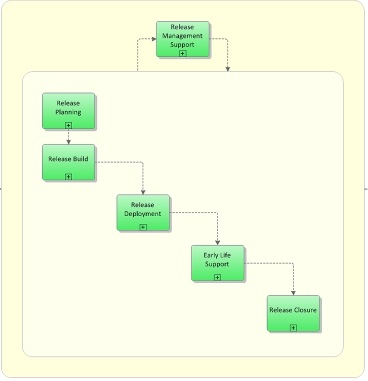
\includegraphics[scale=0.5]{immagini/rollout/release-deployment}
				\caption{Sottoprocessi di Release and Deployment Management (\url{https://goo.gl/7jCkZH}).}
			\end{figure}
         
            
            Il processo è suddiviso nei seguenti sotto-processi:
            \begin{itemize}
            	\item \textbf{Release Management Support:} fornisce linee guida e supporto per lo sviluppo delle release.
                \item \textbf{Release Planning:} assegna le change, dopo che sono state autorizzate, ai release packages e definisce la portata e i contenuti delle release. Inoltre, sviluppa uno schedule per build, test e deployment della release.
                \item \textbf{Release Build:} emette tutti gli ordini di lavoro e le richieste di acquisto per lo sviluppo interno o l'acquisizione delle componenti della release, in modo da renderli disponibili per la fase di test.
                \item \textbf{Release Deployment:} effettua il deploy delle componenti della release nell'ambiente live. Inoltre, forma gli utenti e il personale operativo e si occupa di rilasciare informazioni e documentazione sulle release di cui è stato fatto il deploy.
                \item \textbf{Early Life Support:} risolve problemi operativi nel periodo immediatamente successivo al rilascio, in cui è più probabile che essi si manifestino. Ricordiamo che durante l'Early Life Support il Service Transition affianca il Service Operations.
                \item \textbf{Release Closure:} si occupa della chiusura formale di una release dopo essersi assicurati che i log e il CMDB siano stati aggiornati.
            \end{itemize}

			È molto importante notare come in ITIL V3, rispetto alla versione precedente, siano state create interfacce aggiuntive tra i processi di \textbf{Release Management} e \textbf{Project Management (Transition Planning and Support)}, in modo da assicurarsi che i due processi siano allineati per quanto riguarda l'allocazione di risorse e la pianificazione di attività.
            
            
            La stesura del piano di rollout terrà in considerazione quanto appena esposto: non si limiterà ad essere una semplice pianificazione di attività su calendario, ma verranno descritte, nei limiti del possibile, le attività, suddividendole in compiti (tasks), e le risorse necessarie per portarle a termine con successo.
            
            \subsection{Assunzioni}
            	Data la natura di progetto universitario del documento, nel seguito del documento verrà considerata la seguente assunzione:
                \begin{itemize}
                	\item Una precisa e puntuale quantificazione delle risorse necessarie alla fornitura del servizio, tenendo conto anche gli obiettivi di crescita a medio e lungo termine, dovrebbe essere eseguita dal processo di Capacity Management, che non viene istanziato nel presente documento, tenendo conto anche di analisi più approfondite dell'ambiente del Proponente. In ogni caso, l'Offerente cercherà di effettuare delle stime iniziali di risorse. 
                \end{itemize}
                
                
		\subsection{Riferimenti}
        	Il piano di rollout prenderà spunto dal seguente template, che guida la stesura di un Project Implementation Plan:
            \begin{itemize}
            	\item \texttt{Project Implementation Plan template: \url{https://goo.gl/LSGktb}}. 
            \end{itemize}
            
            Inoltre, il piano verrà integrato seguendo altri template e verranno presi spunti e informazioni da altre fonti. Tutti questi riferimenti sono indicati di seguito:
       		\begin{itemize} 
            	\item \texttt{Rollout Plan, Frank Bergmann: \url{http://project-open.sourceforge.net/whitepapers/Project-Open-Rollout-Plan.pdf}}.
                \item \texttt{Mifos - Pilot and Rollout Plan, Grameen Foundation: \url{https://goo.gl/TcjL4s}}.
                \item \texttt{Project Charter for MoHSS HRIMS Rollout Project : \url{https://www.ihris.org/toolkit-new/scale-up/example-rollout-plan/}}.
				\item \texttt{Processo di Release and Deployment Management del framework ITIL V3: \url{https://wiki.en.it-processmaps.com/index.php/Release_and_Deployment_Management}}.
                \item \texttt{Big bang ERP implementation vs phased approach, pros and cons: \url{https://goo.gl/7M7JmS}}.
                \item \texttt{Regolamento sulla privacy 2018: \url{https://www.laleggepertutti.it/227787_privacy-cosa-cambia-a-maggio-2018}}.
                \item \texttt{Privacy by default e by design: \url{https://protezionedatipersonali.it/privacy-by-design-e-by-default}}.
                \item \texttt{Security and Privacy: an introduction to ISO 27000: \url{https://iapp.org/media/presentations/14Symposium/CS14_Introduction\%20to\%20ISO.pdf}}.
                \item \texttt{A Qualitative Risk Analysis and Management Tool: CRAMM: \url{https://goo.gl/uZzqv9}}.
                
                \item \texttt{A Processo di Service Validation and Testing del framework ITIL V3: \url{https://wiki.en.it-processmaps.com/index.php/Service_Validation_and_Testing}}.
			\end{itemize}
            
		\newpage
%**************************** SEZIONE 2: PANORAMICA GENERALE *******************
%*
%*
%*
	\section{Panoramica di gestione}
    	In questa sezione verranno descritte le dinamiche di gestione per l'implementazione della soluzione, identificando le attività principali e suddividendole in compiti (tasks).
		
        \subsection{Descrizione dell'implementazione}
			L'implementazione della soluzione seguirà le seguenti fasi:
            \begin{itemize}
            	\item \textbf{Definizione:} in questa fase verranno:
                \begin{itemize} 
                	\item Identificati, discussi e approvati i moduli che dovranno essere implementati.
                    \item Identificate le eventuali necessità di estensione.
                    \item Specificate le necessità di configurazione e personalizzazione.
                    \item Identificati i requisiti della soluzione.
                \end{itemize}
                \item \textbf{Estensione:} questa fase concerne:
                \begin{itemize}
                	\item La realizzazione di mockup iniziali per i sistemi e le applicazioni da realizzare.
                    \item La definizione di come le eventuali estensioni richieste andranno ad impattare i moduli esistenti.
                    \item L'implementazione delle estensioni richieste.
                    \item La realizzazione e la presentazione al Proponente di un prototipo.
                    \item Il completamento del prototipo e il test nell'ambiente del Proponente.
                    \item La realizzazione di documentazione tecnica e di materiale per gli utenti (manuali, ecc).
                \end{itemize}
                \item \textbf{Installazione:} durante questa fase verranno:
                \begin{itemize}
                	\item Installate le soluzioni su ambienti di produzione, di sviluppo e di test.
                    \item Configurate le soluzioni in base alle necessità di configurazione e personalizzazione definite precedentemente.
                    \item Impostati i profili utenti e assegnati i privilegi correttamente.
                    \item Importati i dati necessari al funzionamento della soluzione.
                \end{itemize}
                \item \textbf{Formazione:} in questa fase l'Offerente affiancherà il Proponente, fornendo formazione agli utenti in modo da renderli in grado di utilizzare correttamente la soluzione.
                \item \textbf{Go-live:} questa fase prevede:
                \begin{itemize}
                	\item  L'ottenimento dell'autorizzazione di entrambi Proponente e Offerente per andare live.
                    \item Trasferimento finale dei dati dal vecchio sistema a quello nuovo.
                \end{itemize}
                \item \textbf{Affiancamento:} durante il primo periodo questa fase l'Offerente affianca il Proponente, fornendo parte del team che ha lavorato all'implementazione della soluzione per risolvere dubbi, perfezionare la formazione e aiutare nell'identificazione e risoluzione di incidenti e problemi. Successivamente, si passa al periodo di supporto solamente tramite service desk.
            \end{itemize}
            

            La tipologia di rollout che verrà impiegata è di tipo \textbf{orizzontale/big bang}. Il rollout orizzontale consiste nel far adottare il nuovo sistema a tutta l'azienda nello stesso momento ("go-live"). L'alternativa a questa tipologia è il rollout verticale/phased, che prevede un rollout graduale del sistema, suddividendolo per modulo, business unit o area geografica.


            I vantaggi dell'approccio orizzontale sono:
            \begin{itemize}
            \item Tempo di implementazione più breve.
            \item Non ci sono mai due sistemi diversi utilizzati in contemporanea all'interno dell'azienda.
            \item Possibilità di creare hype in attesa del rilascio del nuovo sistema.
            \item Possibilità di concentrare la formazione esclusivamente sul nuovo sistema.
            \item Minori costi complessivi, dato che il vecchio sistema viene dismesso più in fretta.
            \end{itemize}
            Tuttavia, sono presenti anche alcuni svantaggi:
            \begin{itemize}
            \item I test di sistema sono difficili da eseguire prima del go-live.
            \item Nessuna possibilità di fall-back affidabile nel lungo periodo (dopo la dismissione del vecchio sistema).
            \item Cambiamento improvviso di abitudini di lavoro.
            \item Diminuzione temporanea di produttività.
            \end{itemize}
            Per quanto riguarda il rollout verticale, i vantaggi sono:
            \begin{itemize}
            \item Maggior facilità e minor tempo di adattamento al nuovo sistema.
            \item Possibilità di scoprire i problemi prima e risolverli in modo graduale.
            \item Maggior tempo per poter fare formazione.
            \end{itemize}
            Invece, gli svantaggi sono:
            \begin{itemize}
            \item Costi di implementazione più alti, a causa della coesistenza parziale di due sistemi diversi e dalla necessità di creazione di interfacce per favorire l'intercomunicazione.
            \item Possibilità di invalidare la conformità del sistema complessivo, a causa di incoerenze tra i due sistemi.
            \item Difficoltà di integrazione.
            \end{itemize}
            Alla luce di quanto esposto, nonostante l'approccio generale sarà di tipo orizzontale, l'Offerente ritiene di poter sfruttare un approccio verticale durante la fase di testing. Infatti sarà possibile far testare il sistema applicativo alle singole aree (Sanitaria, Amministrativa, Direzionale, Servizi) un'area alla volta, per poter effettuare formazione preventiva e identificare e risolvere in fretta eventuali problemi.
           
           
		\subsection{Punti di contatto}
        In questa sezione è possibile trovare i contatti dei membri principali del team dell'Offerente che si occuperà dell'implementazione della soluzione.
        \begin{table}[H]
        	%\renewcommand\arraystretch{1,5}
            \begin{tabular}{ c c c }
            \toprule
            \textbf{Ruolo} & \textbf{Nome} &\textbf{Numero di telefono} \\
            \toprule
            Capo progetto & Nome Cognome & 333 666444 \\
            Responsabile privacy & Nome Cognome & 333 666444 \\
            Responsabile qualità & Nome Cognome & 333 666444 \\
            Amministratore database & Nome Cognome & 333 666444 \\
            Responsabile analisi & Nome Cognome & 333 666444 \\
            Responsabile progettazione & Nome Cognome & 333 666444 \\
            \bottomrule
            \end{tabular}
            \caption{Punti di contatto}
        \end{table}

		\subsection{Attività principali}
        \label{sec:attivita}
        	In questa sezione verranno descritte le attività principali necessarie alla corretta implementazione della soluzione. Per ogni attività verranno indicate le seguenti informazioni:
            \begin{itemize}
            	\item \textbf{Deliverables:} oggetti materiali o immateriali risultanti dall'esecuzione dell'attività.
                \item \textbf{Risorse:} le risorse necessarie per l'esecuzione dell'attività.
                \item \textbf{Responsabili:} le persone (inteso come ruoli) chiave responsabili dell'attività.
                \item \textbf{Criteri di accettazione:} criteri per considerare un'attività conclusa con successo.
            \end{itemize}
            Inoltre, quando ritenuto necessario, l'attività verrà suddivisa in compiti (tasks) aventi maggiore granularità. Verranno inoltre utilizzati diagrammi di attività del linguaggio di modellazione UML3 per descrivere con maggiore precisione il flusso di esecuzione.
            
            \subsubsection{Subentro contrattuale}
            	Il Proponente desidera passare da una fornitura con service provider multipli ad una fornitura di tipo \textit{sole provider}. L'Offerente deve quindi prendere in carico la gestione di tutti i contratti esistenti alla data di aggiudicazione dell'appalto. L'Offerente reputa fondamentale avvisare i fornitori del Proponente di questa presa in carico. Nel caso in cui il fornitore non dovesse dare il benestare, l'Offerente avvertirà il Coordinatore di Progetto dell'accaduto allo scopo di prendere una decisione per risolvere la situazione.
                \begin{figure}[H]
                  	\centering
                  	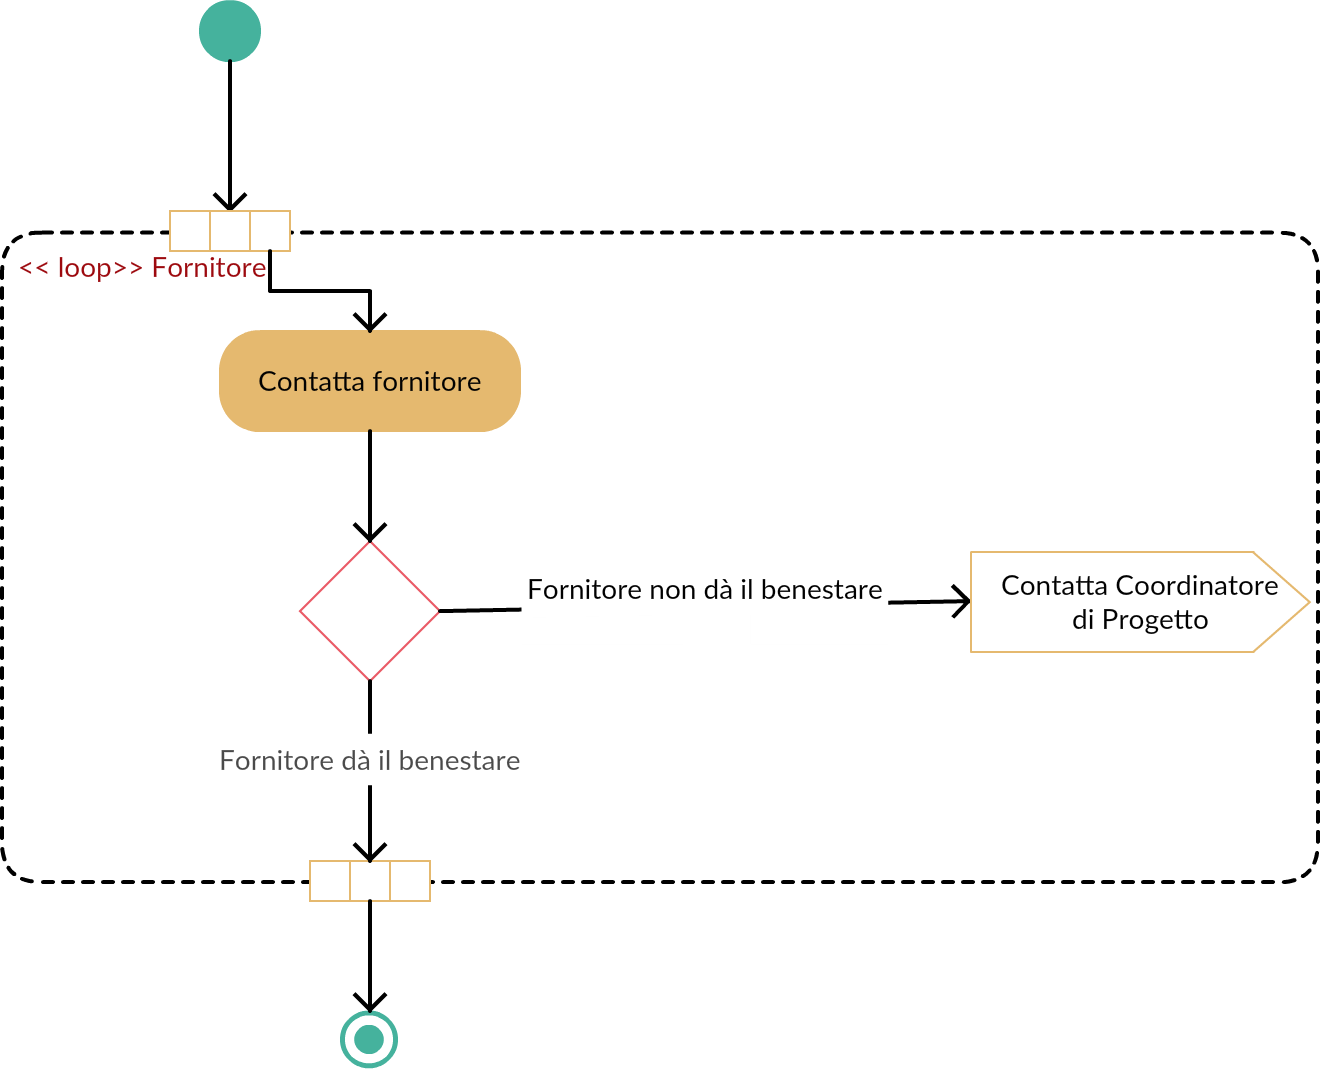
\includegraphics[scale=0.25]{immagini/rollout/contatta-fornitore}
                	\caption{Diagramma di attività del subentro contrattuale.}
				\end{figure}
                
                 \begin{itemize}
               		\item  \textbf{Deliverables:} subentro completato per tutti i contratti esistenti.
                    \item  \textbf{Risorse:} una persona.
                    \item  \textbf{Responsabili:} Capo Progetto.
                    \item  \textbf{Criteri di accettazione:} benestare da parte di tutti i service provider.
                \end{itemize}
            
            
            \subsubsection{Business Process Reengineering (BPR)}
				L'attività di BPR tratta una profonda revisione dei processi aziendali, che ricordiamo essere insiemi di attività correlate che producono valore trasformando degli input in determinati output. La richiesta del Proponente infatti non si limita a richiedere solamente una soluzione tecnologica: il suo obiettivo è la trasformazione del modello aziendale da gerarchico-funzionale a un modello per processi, caratterizzato da una maggiore integrazione.
                \begin{figure}[H]
                  	\centering
                  	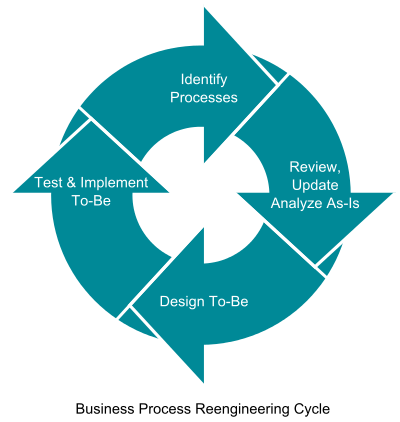
\includegraphics[scale=0.4]{immagini/rollout/BPR}
                	\caption{Ciclo di BPR (\url{https://goo.gl/1Vdufy}).}
				\end{figure}
                Si può suddividere l'attività di BPR in quattro fasi:
                \begin{enumerate}
                	\item \textbf{Identificazione dei processi:} durante questa fase è necessario identificare i processi esistenti (\textit{as-is}) per avere le informazioni di base da cui partire.
                    \item \textbf{Revisione, aggiornamento e analisi dell'as-is:} in questa fase è necessario analizzare in profondità i processi identificati, allo scopo di avere più informazioni possibili.
                    \item \textbf{Design to-be:} in questa fase vengono progettati i nuovi processi, seguendo le linee guida e gli obiettivi del Proponente.
                    \item \textbf{Test e implementazione del to-be}: in quest'ultima fase i processi vengono testati ed effettivamente implementati nella realtà aziendale del Proponente.
                \end{enumerate}
                    
                \begin{itemize}
               		\item  \textbf{Deliverables:} documento Organizzazione dei Processi Aziendali.
                    \item  \textbf{Risorse:} 
                    \begin{itemize}
                    	\item Due persone per l'analisi e lo sviluppo dei processi.
                        \item Due computer portatili.
                        \item Due licenze Microsoft Office.
                    \end{itemize}
                    \item  \textbf{Responsabili:} analisti con conoscenza di processi aziendali.
                    \item  \textbf{Criteri di accettazione:} accettazione da parte del Proponente.
                \end{itemize}

                \subsubsection*{Tasks}
					\begin{enumerate}
						\item \textbf{Osservazione del modo di lavorare presso il Proponente}.\\
                        Per poter analizzare i processi nel dettaglio è necessario presenziare di persona presso la sede del Proponente, per ottenere più informazioni possibili. Il personale dell'Offerente comincerà ad essere presente nella sede del Proponente fin da subito e stilerà relazioni quindicinali su quanto appreso.
					\end{enumerate}
                    
			\subsubsection{Presa in carico sistemi ed erogazione servizi esistenti}  
            	Il Proponente desidera che l'Offerente prenda in carico i sistemi esistenti, prestando parte attiva nell'erogazione dei servizi fin da subito, e non limitandosi esclusivamente allo sviluppo di una soluzione da rilasciare in futuro. 
                \begin{itemize}
                \item \textbf{Deliverables:} 
                	\begin{itemize}
                    	\item Documento Analisi Sistemi.
                    	\item Sistemi presi in carico correttamente.
                        \item Servizi esistenti erogati correttamente.
                    \end{itemize}
                \item  \textbf{Risorse:} 
                \begin{itemize}
                	\item Personale del Centro Gestione Integrato (comprende il Service Desk).
                	\item Hardware esistente presso la sede del Proponente.
                    \item Software esistente presso la sede del Proponente.
                    \item Fornitori attuali del Proponente.
                \end{itemize}
                \item  \textbf{Responsabili:} Personale del Centro Gestione Integrato, Capo Progetto.
                \item  \textbf{Criteri di accettazione:} 
                \begin{itemize}
					\item Test dei sistemi attualmente esistenti.
                    \item Test di erogazione dei servizi esistenti.
                \end{itemize}
                \end{itemize}
                Il seguente diagramma di attività mostra una visione più granulare dell'attività, concentrandosi sulla presa in carico dei sistemi. La presa in carico dei servizi verrà eseguita in modo similare.
                \begin{figure}[H]
					\centering
					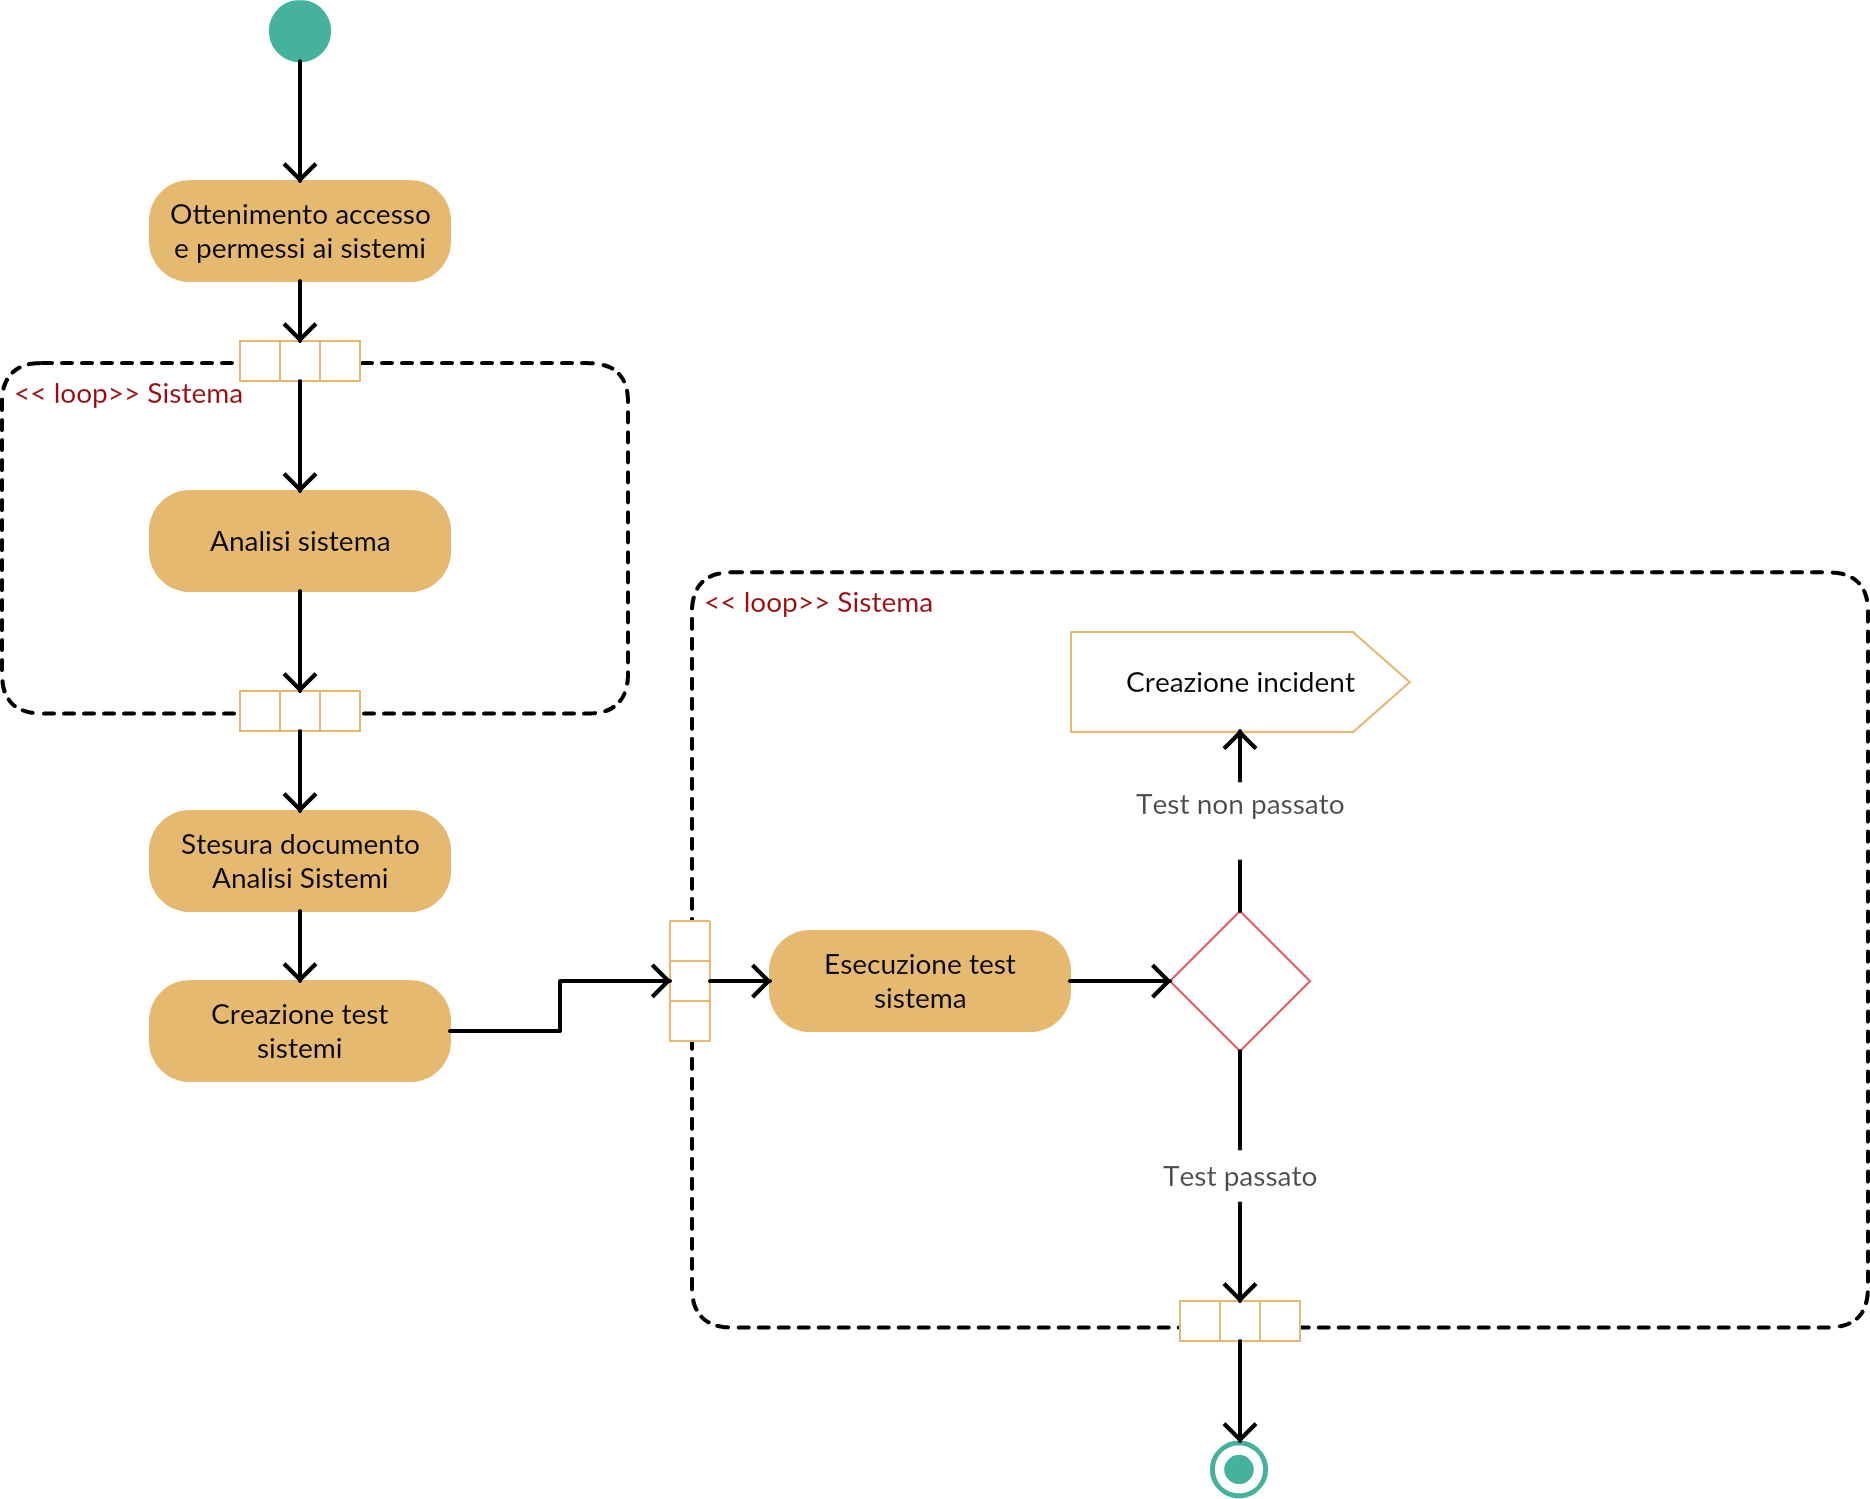
\includegraphics[width=\textwidth]{immagini/rollout/carico-sistemi}
					\caption{Diagramma di attività della presa in carico dei sistemi.}
				\end{figure}
                
                    \subsubsection*{Tasks}
					\begin{enumerate}
                    
                    	 \item \textbf{Ottenimento accesso e permessi di amministratore ai sistemi esistenti}.\\
                         Ottenere l'accesso e i permessi di amministratore per i sistemi esistenti è il primo passo da eseguire.
						\item \textbf{Analisi sistemi esistenti}.\\
                        Analizzare e comprendere i sistemi esistenti presso la sede del Proponente è il passo successivo verso una presa in carico efficace. L'Offerente si occuperà della stesura di un documento di Analisi Sistemi.
                       \item \textbf{Analisi servizi esistenti}.\\
                        Oltre ai sistemi, è necessario analizzare anche i servizi, per comprenderne al meglio le logiche di erogazione.
                       \item \textbf{Test dei sistemi}.\\
                        Prima di poter erogare un servizio l'Offerente vuole accertarsi che i sistemi rispondano correttamente. Per questo motivo, verranno eseguiti dei test per valutare l'adeguatezza di ogni sistema.
                        \item \textbf{Test di erogazione servizi}.\\
                        Una volta essersi assicurati che i sistemi siano adeguati, l'Offerente effettuerà un test di erogazione per ogni servizio, coinvolgendo anche il personale del Proponente.
					\end{enumerate}
                
			\subsubsection{Riprogettazione e reimplementazione Centro Elaborazione Dati (CED)}
				L'Offerente ha scelto di ospitare tutto l'hardware necessario presso il CED del proponente. Tuttavia, il CED ha bisogno di una profonda riprogettazione, sia dal punto di vista hardware, sia per quanto riguarda la messa a norma. L'Offerente non esclude la necessità di interventi strutturali al CED.
                
                \begin{itemize}
               		\item  \textbf{Deliverables:} CED riprogettato e reimplementato.
                    \item  \textbf{Risorse} 
                    \begin{itemize}
                    	\item Due persone per l'analisi, la riprogettazione e la reimplementazione del CED.
                        \item Azienda esterna per interventi strutturali, qualora ce ne fosse bisogno.
                        \item Hardware (porte tagliafuoco, armadi ignifughi, server, ecc) e software necessari.
                	\end{itemize}
                    \item  \textbf{Responsabili:} persone con buone capacità progettuali e conoscenze di networking. 
                    \item  \textbf{Criteri di accettazione:} 
                    \begin{itemize}
                    	\item Test di sistema per valutare la funzionalità del nuovo CED.
                        \item Accettazione da parte del Proponente.
                    \end{itemize}
                \end{itemize}
                
                \subsubsection*{Tasks}
                	\begin{enumerate}
                		\item \textbf{Analisi CED attuale:} analizzare la situazione corrente è fondamentale per capire le funzionalità richieste dal CED.
                        \item \textbf{Progettazione nuovo CED:} dopo che è stata svolta l'analisi, è necessario progettare il nuovo CED, sia dal punto di vista strutturale, sia dal punto di vista di hardware e software.
                        \item \textbf{Esecuzione lavori strutturali:} solo se necessario, dovranno essere eseguiti lavori strutturali (allargamento locale, sistemazione muratura, ecc).
                        \item \textbf{Installazione hardware e software:} verranno installati hardware e software identificati durante la progettazione.
                        \item \textbf{Test del nuovo CED:} verrà eseguito un test dell'intero CED per valutare la corretta implementazione di tutte le funzionalità richieste. Il collaudo verrà eseguito con l'assistenza del personale tecnico dell'U.O. Gestione Tecnico-Patrimoniale, come segnalato nel Capitolato. 
                	\end{enumerate}
                    
			\subsubsection{Personalizzazione e implementazione SAP}
            	L'Offerente ritiene che l'adozione di un ERP sia la soluzione migliore per raggiungere gli obiettivi di integrazione, re-ingegnerizzazione dei processi aziendali e riduzione del numero di applicazioni e sistemi richiesti dal Proponente. L'ERP scelto dall'Offerente è SAP, un software ERP che permette una profonda personalizzazione per meglio adattarlo alla propria realtà e processi aziendali.
                Un software come SAP non è pronto \textit{out-of-the-box}: è necessario eseguire vari passi prima di poterne effettuare il deployment, che verranno descritti dai tasks successivi.
                \begin{itemize}
               		\item  \textbf{Deliverables:} ERP SAP correttamente personalizzato e implementato.
                    \item  \textbf{Risorse:} 
                    \begin{itemize}
                    	\item Tre persone per analisi, progettazione, implementazione e test delle personalizzazioni di SAP.
                        \item Licenze SAP.
                        \item PC, server e sistemi necessari per lo sviluppo e l'installazione di SAP.
                	\end{itemize}
                    \item  \textbf{Responsabili:} analisi, progettisti e programmatori.
                    \item  \textbf{Criteri di accettazione:} 
                    \begin{itemize}
                    	\item Test di sistema di SAP.
                        \item Accettazione da parte del Proponente.
                    \end{itemize}
                \end{itemize}
                
                \subsubsection*{Tasks}
                	\begin{enumerate}
                		\item \textbf{Analisi requisiti:} il primo passo da compiere è analizzare i requisiti e le funzionalità che SAP deve implementare. Più nel dettaglio, dato che il Proponente vuole passare da una situazione con numerosi applicativi ad una con un numero ristretto di applicativi, è necessario analizzare con precisione le funzionalità delle applicazioni attualmente esistenti, per poterle replicare in SAP.
                        \item \textbf{Progettazione personalizzazioni:} dopo aver eseguito l'analisi, è fondamentale progettare le personalizzazioni necessarie.
                        \item \textbf{Implementazione personalizzazioni:} una volta progettate, le personalizzazioni devono essere implementate.
                        \item \textbf{Integrazione CRS-SISS:} date le richieste del Proponente in ambito di integrazione con i progetti sanitari regionali, sarà necessario integrare SAP con il progetto CRS-SISS.
                        \item \textbf{Test di sistema:} una volta completate tutte le attività di implementazione, sarà necessario testare SAP per verificarne la conformità ai requisiti identificati.
                        \item \textbf{Migrazione dati applicativi in SAP:} l'ultimo passo prima di poter utilizzare SAP operativamente è eseguire la migrazione dei dati degli applicativi esistenti.
                	\end{enumerate}
                    
                    
                \subsubsection{Revisione cablaggio e architettura di rete}
	La situazione dell'architettura di rete presso la sede del Proponente presenta diverse problematiche, come tratti con cablaggio a bassa velocità (inferiori al Gigabit) e tratti che bypassano il centro stella, per collegarsi direttamente al CED (come il collegamento dal Servizio Traumatologico d'Urgenza STU).
                    Inoltre, il centro stella risulta attualmente non ridondato, diventando quindi un \textit{single point of failure}.
                    
                    
                    Per ottenere una rete solida, ridondata e senza \textit{single point of failure} sarà necessario eseguire i task descritti più in basso.
                    
                    \begin{itemize}
               		\item  \textbf{Deliverables:} 
                    \begin{itemize}
                    	\item Nuova rete correttamente progettata e implementata.
                        \item Documento Piano di indirizzamento IP e di partizionamento della rete.
                    \end{itemize}
                   
                    \item  \textbf{Risorse} 
                    \begin{itemize}
                    	\item Due persone per analisi, progettazione architettura di rete.
                        \item Azienda esterna per esecuzione lavori di cablaggio e/o ricertificazione fibra, se ritenuto necessario.
						\item Hardware necessario (cavi, router, switch, ecc).
                	\end{itemize}
                    \item  \textbf{Responsabili:} progettisti di rete.
                    \item  \textbf{Criteri di accettazione:} 
                    \begin{itemize}
                    	\item Test di sistema sulla funzionalità di rete.
                        \item Test di ridondanza sulla rete.
                        \item Accettazione da parte del Proponente.
                    \end{itemize}
                	\end{itemize}
                    
                    \subsubsection*{Tasks}
                	\begin{enumerate}
                		\item \textbf{Analisi rete attuale:} il primo passo da eseguire è l'analisi della rete attuale.
                        \item \textbf{Stesura documento Piano di indirizzamento IP e di partizionamento della rete:} questo documento descriverà come l'Offerente intende organizzare l'indirizzamento degli IP e progettare la rete.
                        \item \textbf{Implementazione nuova rete:} sarà necessario eseguire lavori per il cablaggio di nuovi cavi e ricertificazione per quelli esistenti.
                        \item \textbf{Test nuova rete:} sarà necessario infine testare la nuova rete con test che ne verifichino sia la corretta funzionalità che le caratteristiche di ridondanza.
                	\end{enumerate}
                    
                    \subsubsection{Costituzione Centro di Gestione Integrato (CGI)}
                    	Il Proponente desidera la costituzione di un Centro di Gestione Integrato (CGI) presso la propria sede. Lo scopo del CGI è di fornire un servizio dedicato di gestione e assistenza alla struttura ospedaliera.
                        
                        
                        Il CGI sarà composto da:
                        \begin{enumerate}
                        	\item Service Desk.
                            \item Centro di Controllo e Monitoraggio.
                            \item Servizi On-Site per le postazioni di lavoro.
                            \item Risorse in reperibilità notturna e festiva.
                            \item Centro di Supporto per l'Area Direzionale.
                            \item Centro di Supporto per l'Area Gestione Personale.
                        \end{enumerate}
                        
                        
                        \begin{itemize}
               		\item  \textbf{Deliverables:} 
                    \begin{itemize}
                    	\item Centro di Gestione Integrato operativo.
                        \item Documento Organizzazione Centro di Gestione Integrato.
                    \end{itemize}
                                       
                    \item  \textbf{Risorse:} 11 persone in totale, suddivise nel seguente modo: 
                    \begin{itemize}
                    	\item 5 persone per il Service Desk.
                        \item 2 persone per il Centro di Controllo e Monitoraggio.
                        \item 2 persone per i Servizi On-Site per le postazioni di lavoro.
                        \item 2 persone in reperibilità notturna e festiva, a rotazione tra quelle presenti all'interno del CGI.
                        \item 1 persona per il Centro di Supporto per l'Area Direzionale.
                        \item 1 persona per il Centro di Supporto per l'Area Gestione Personale.
                	\end{itemize}
                    \item  \textbf{Responsabili:} 
                    \begin{itemize}
                    	\item Persone con buone capacità di problem solving.
                        \item Persone con buone conoscenze IT per quanto riguarda le postazioni di lavoro.
                        \item Persone con conoscenze di management per il supporto all'area direzionale.
                        \item Persone con conoscenze in ambito di gestione personale.
                    \end{itemize}
                    \item  \textbf{Criteri di accettazione:} 
                    \begin{itemize}
                        \item Accettazione da parte del Proponente.
                    \end{itemize}
                	\end{itemize}
                
                    \subsubsection{Presa in carico postazioni di lavoro}
                    	Le postazioni di lavoro attualmente presenti presso la sede del Proponente sono estremamente variabili per quanto riguarda marca e anno di acquisto. Inoltre, le informazioni riguardo la marca per alcune postazioni di lavoro risultano non essere disponibili: questo è sintomo di un processo di Service Asset and Configuration Management svolto in maniera non ottimale.
                        
                        
                        L'Offerente desidera prendere in carico, come richiesto, la gestione delle postazioni di lavoro, risolvendo le problematiche segnalate e successivamente controllando e sostituendo regolarmente le postazioni di lavoro.
                        
                        
                        Il diagramma di attività sottostante mostra il flusso di lavoro della sostituzione di una postazione di lavoro. Il diagramma per sostituzione stampanti e altro hardware è similare, con l'accortezza di cambiare il limite temporale da prendere in considerazione per la sostituzione.
                        \begin{figure}[H]
							\centering
							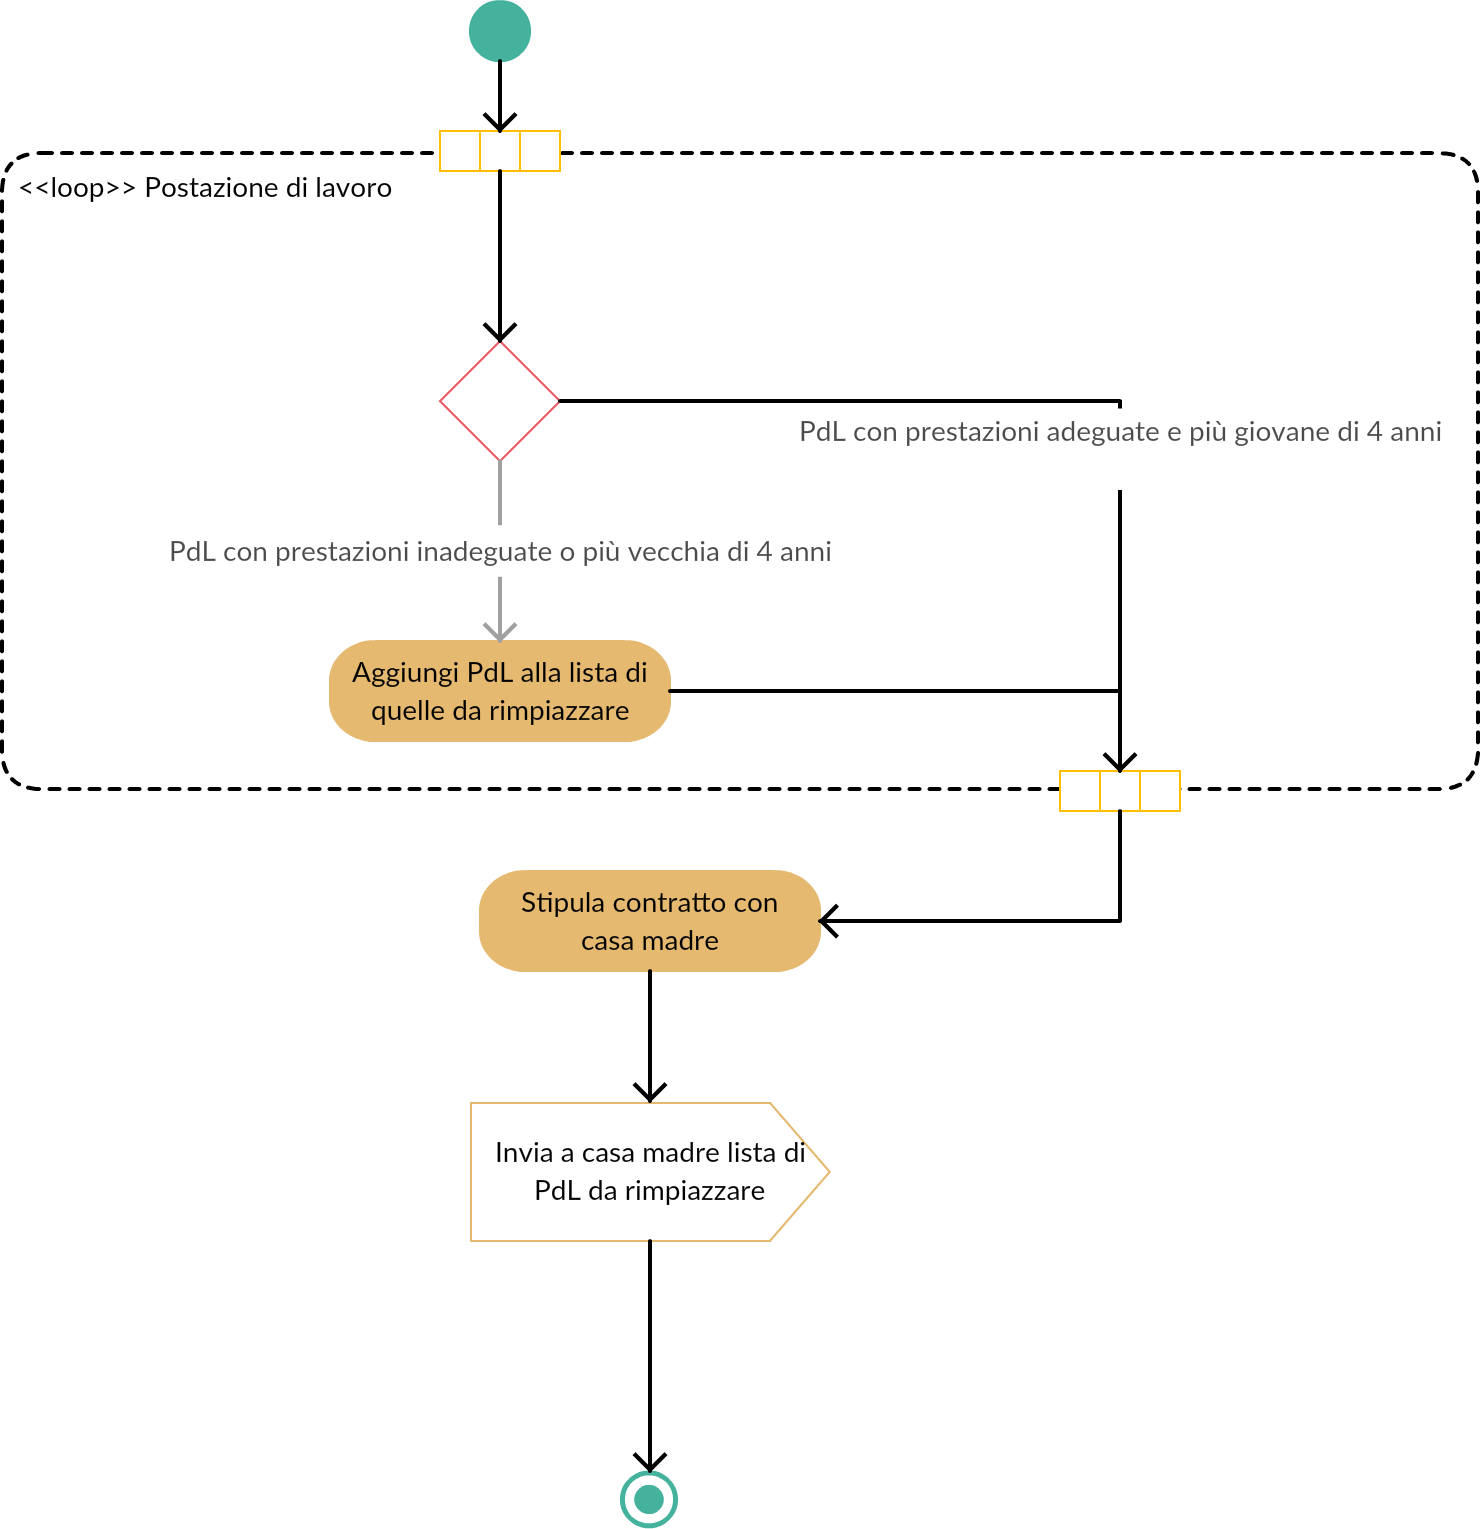
\includegraphics[scale=0.237]{immagini/rollout/sostituzione-pdl}
							\caption{Diagramma di attività sostituzione PdL.}
							\end{figure}
                        
                        
                        
                         \begin{itemize}
               		\item  \textbf{Deliverables:} 
                    \begin{itemize}
                    	\item Postazioni di lavoro troppo vecchie o inadeguate rimpiazzate.
                        \item Postazioni di lavoro gestite completamente dall'Offerente.
                    \end{itemize}
                                       
                    \item  \textbf{Risorse:} 
                	\begin{itemize}
                		\item Postazioni di lavoro, stampanti e altro hardware e software necessari. 
                        \item Azienda esterna (casa madre) che si occupi dell'installazione e manutenzione.
                	\end{itemize}
                    \item  \textbf{Responsabili:} azienda esterna (casa madre).
                    \item  \textbf{Criteri di accettazione:} 
                    \begin{itemize}
                    	\item Nessuna postazione di lavoro più vecchia di 4 anni rimanente.
                        \item Nessuna stampante a getto d'inchiostro o ad aghi più vecchia di 18 mesi rimanente.
                        \item Nessuna stampante laser più vecchia di 2 anni rimanente.
                        \item Nessuna stampante laser dipartimentale più vecchia di 4 anni rimanente.
                    \end{itemize}
                	\end{itemize}
                    
                    \subsubsection*{Tasks}
                    \begin{enumerate}
                    	\item \textbf{Identificazione postazioni di lavoro da sostituire:} è necessario identificare le PdL con prestazioni inadeguate o troppo vecchie e aggiungerle alla lista per la sostituzione.
                        \item \textbf{Stipulazione contratto:} è necessario stipulare un contratto con una ditta esterna (possibilmente casa madre) per l'acquisto, l'installazione e la manutenzione delle PdL da sostituire.
                    \end{enumerate}
                    
			\subsubsection{Sviluppo progetti innovativi}
            	Il Proponente, con lo scopo di mantenere alto il proprio livello di competitività e innovazione tecnologica, richiede lo sviluppo di progetti innovativi. Dato che questi progetti possono richiedere tecnologie innovative, l'Offerente prevede di appoggiarsi anche a figure come ricercatori e dottorandi nella fase di ideazione.
                
                \begin{itemize}
               		\item  \textbf{Deliverables:} 
                    \begin{itemize}
                    	\item Progetti innovativi sviluppati e implementati correttamente.
                        \item Documento Progetti Innovativi.
                    \end{itemize}
                                       
                    \item  \textbf{Risorse:} 
                	\begin{itemize}
                		\item 2 persone quali dottorandi e ricercatori per la fase di ideazione.
                        \item 3 persone interne all'Offerente per progettazione e implementazione.
                	\end{itemize}
                    \item  \textbf{Responsabili:} figure con buone capacità innovative e mente aperta.
                    \item  \textbf{Criteri di accettazione:} 
                    \begin{itemize}
                    	\item Test di sistema per ogni progetto innovativo.
                        \item Accettazione da parte del proponente.
                    \end{itemize}
                	\end{itemize}
                    
                    \subsubsection*{Tasks}
                    \begin{enumerate}
                    	\item \textbf{Identificazione figure esterne:} come primo passo l'Offerente desidera identificare figure quali dottorandi e ricercatori per l'ideazione dei progetti innovativi.
                        \item \textbf{Brainstorming:} le figure esterne e il team dell'Offerente dovranno eseguire un brainstorming per l'identificazione delle idee innovative.
                        \item \textbf{Scelta idee:} una volta identifica le idee, devono essere valutate e infine scelte quelle ritenute migliori, coinvolgendo anche il Proponente.  
                        \item \textbf{Progettazione:} sarà necessario progettare le soluzioni innovative.
                        \item \textbf{Implementazione:} successivamente alla progettazione, sarà necessario implementare quanto progettato.
                        \item \textbf{Test:} infine, bisognerà testare le soluzioni innovative implementate.
                    \end{enumerate}
                    
                    
			\subsubsection{Stesura documentazione preliminare}
            	Il Proponente richiede la presentazione di documentazione preliminarmente all'assegnazione dell'appalto. La stesura di questa documentazione è molto importante dato che l'Offerente verrà scelto in base al grado di dettaglio, chiarezza e precisione della documentazione.
                
                
                La stesura della documentazione sarà supervisionata dal Capo Progetto.
                \begin{itemize}
               		\item  \textbf{Deliverables:} 
                    \begin{itemize}
                    	\item Documento Presentazione dell'Impresa.
                        \item Documento Progetto Organizzativo.
                        \item Documento Progetto Applicativo.
                        \item Documento Progetto Tecnologico.
                        \item Documento Progetto delle sperimentazioni e delle proposte innovative.
                        \item Documento Progetto di Erogazione e Gestione del Servizio.
                        \item Documento Pianificazione generale.
                    \end{itemize}
                                       
                    \item  \textbf{Risorse:} 
                	\begin{itemize}
                		\item 3 analisti.
                        \item 2 progettisti.
                        \item Capo Progetto.
                	\end{itemize}
                    \item  \textbf{Responsabili:} analisti, progettisti e capo progetto.
                    \item  \textbf{Criteri di accettazione:} 
                    \begin{itemize}
                    	\item Accettazione da parte del Capo Progetto.
                    \end{itemize}
                	\end{itemize}
                    
					\subsubsection*{Tasks}
                    \begin{enumerate}
                    	\item \textbf{Stesura Presentazione dell'Impresa}.
                        \item \textbf{Stesura Progetto Organizzativo}.
                        \item \textbf{Stesura Progetto Applicativo}.
                        \item \textbf{Stesura Progetto Tecnologico}.
                        \item \textbf{Stesura Progetto delle sperimentazioni e delle proposte innovative}.
                        \item \textbf{Stesura Progetto di Erogazione e Gestione del Servizio.}.
                        \item \textbf{Stesura Pianificazione generale}.
                    \end{enumerate}
                    
			\subsubsection{Realizzazione soluzione di continuità}
            	L'Offerente intende garantire la Business Continuity realizzando una soluzione come descritta nel capitolo 2. La soluzione di continuità verrà implementata man mano che i servizi e i sistemi della nuova soluzione andranno live.
                
                
                Maggiori dettagli sull'implementazione della soluzione sono presenti nella sezione \ref{ScadenzaContinuità}.
                
                \begin{itemize}
               		\item  \textbf{Deliverables:} 
                    \begin{itemize}
                    	\item Soluzione di continuità implementata e testata correttamente.
                        \item Sito di Disaster \& Recovery attivo.
					\end{itemize}    
                    \item  \textbf{Risorse:} 
                	\begin{itemize}
                		\item 2 analisti.
                        \item 2 progettisti.
                        \item 1 sistemista.
                        \item Capo Progetto.
                	\end{itemize}
                    \item  \textbf{Responsabili:} analisti, progettisti, sistemisti e Capo Progetto.
                    \item  \textbf{Criteri di accettazione:} 
                    \begin{itemize}
                    	\item Superamento test di sistema.
                    	\item Accettazione da parte del Capo Progetto.
                    \end{itemize}
                	\end{itemize}
                    
					\subsubsection*{Tasks}
                    \begin{enumerate}
                    	\item \textbf{Analisi}.
                        \item \textbf{Progettazione}.
                        \item \textbf{Implementazione}.
                        \item \textbf{Test}.
                    \end{enumerate}
                    
			\subsubsection{Test periodico soluzione di continuità}
            	L'Offerente intende effettuare dei test annuali per garantire l'efficacia operativa della soluzione di continuità. Maggiori dettagli riguardo questi test sono stati descritti nel capitolo 2. 
                
                \begin{itemize}
               		\item  \textbf{Deliverables:} 
                    \begin{itemize}
                    	\item Soluzione di continuità testata correttamente.
                        \item Documento Esito test soluzione di continuità.
					\end{itemize}    
                    \item  \textbf{Risorse:} 
                	\begin{itemize}
                		\item 2 sistemisti.
                	\end{itemize}
                    \item  \textbf{Responsabili:} sistemisti.
                    \item  \textbf{Criteri di accettazione:} 
                    \begin{itemize}
                    	\item Superamento test di sistema.
                    \end{itemize}
                	\end{itemize}
                    
					\subsubsection*{Tasks}
                    \begin{enumerate}
                    	\item \textbf{Test soluzione di continuità}.
                    \end{enumerate}
                    
                    
		\subsection{Pianificazione dell'implementazione e milestones}
        	In questa sezione verrà presentata una pianificazione temporale delle attività identificate nella sezione precedente. Ad ogni attività verrà assegnata:
            \begin{itemize}
            	\item Data d'inizio.
                \item Data di fine.
                \item Durata.
            \end{itemize}
            Inoltre verranno identificate alcune \textit{milestones}, ovvero dei traguardi intermedi importanti per lo svolgimento del progetto.
            
            
            Per motivi di semplicità di rappresentazione, si assumerà che la firma del contratto e la data di verbale di inizio progetto avvengano in data 01/01/n. Naturalmente le attività di redazione di documentazione preliminare e analisi tramite sopralluoghi inizieranno prima della data di presa in carico.
            
            
            Le \textit{milestones} sono identificate tramite dei riquadri sotto il completamento di alcune attività. 
            
            
            \begin{figure}[H]
				\centering
				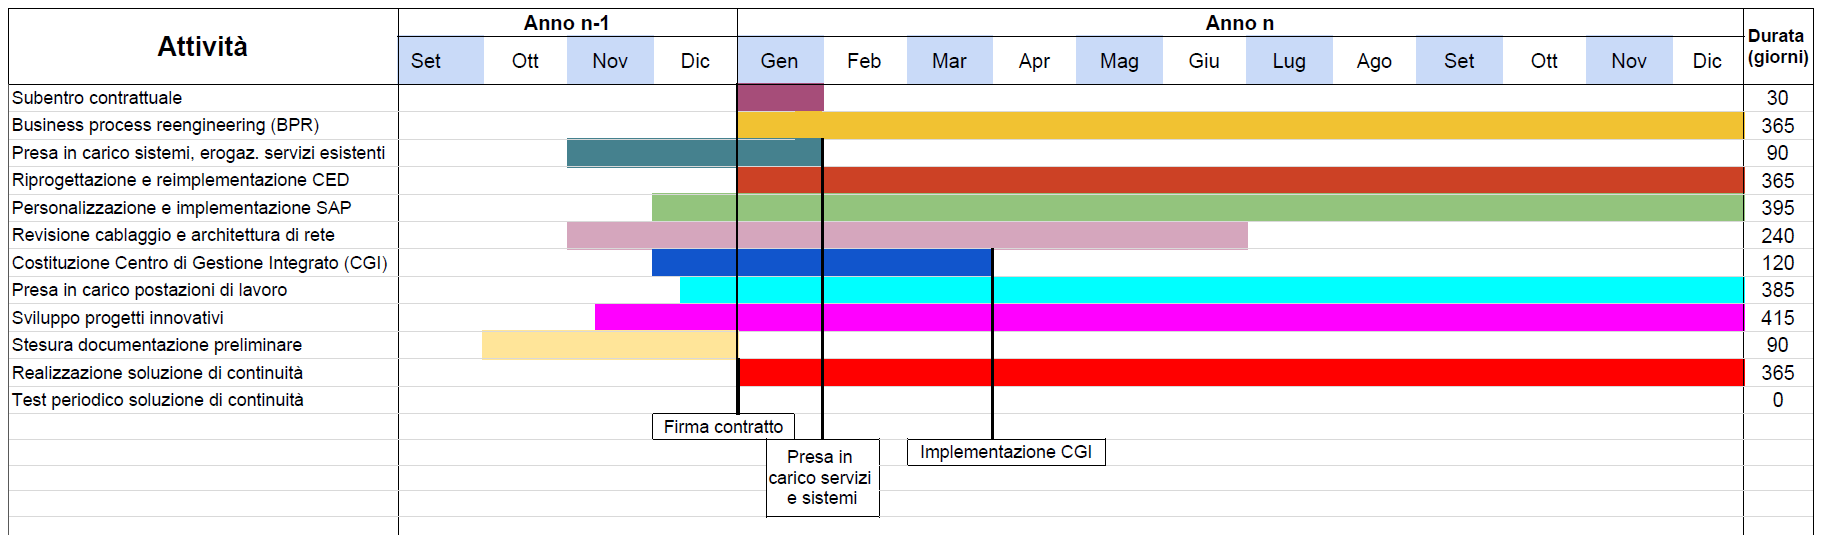
\includegraphics[width=\textwidth]{immagini/rollout/gantt-a1}
				\caption{Gantt anno n-1 e n.}
			\end{figure}
            
            \begin{figure}[H]
				\centering
				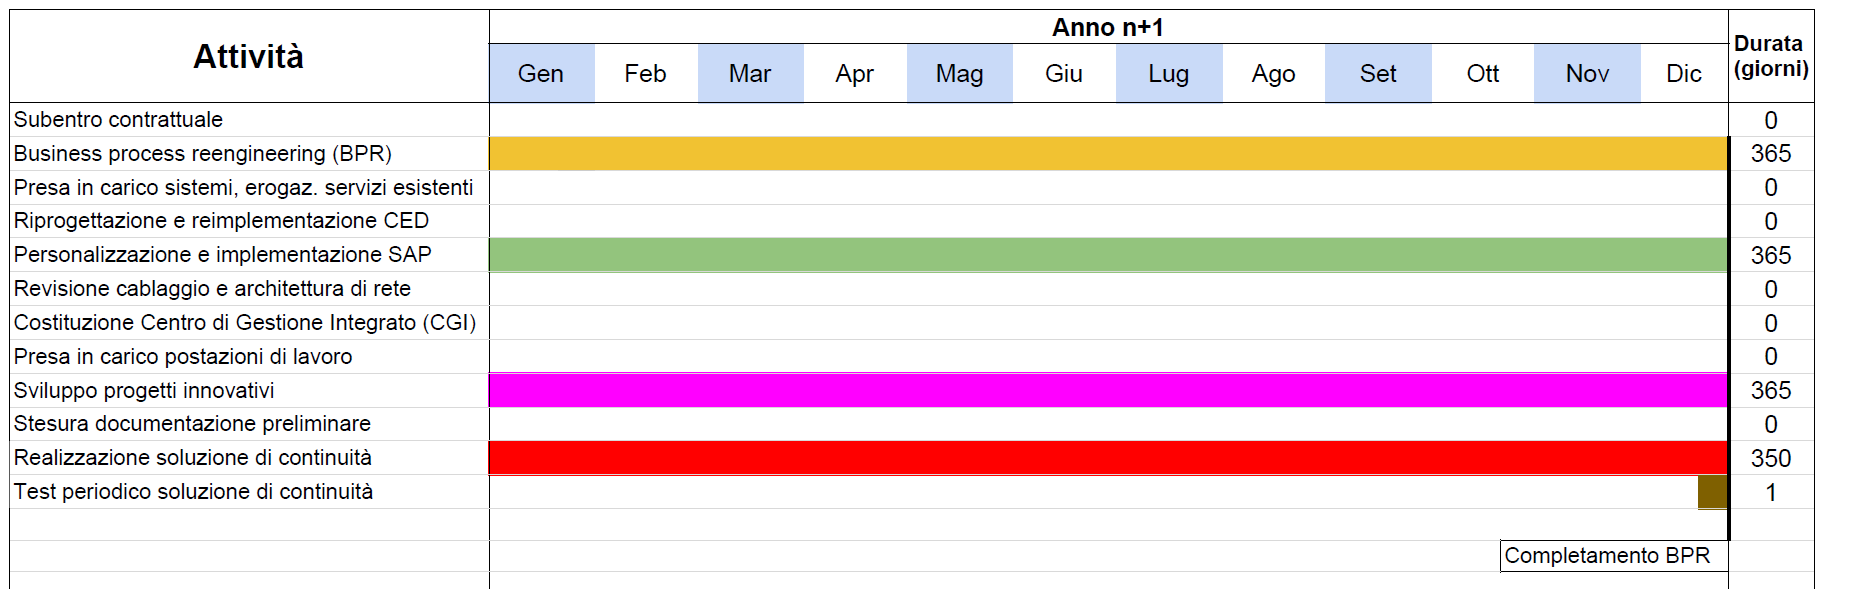
\includegraphics[width=\textwidth]{immagini/rollout/gantt-a2}
				\caption{Gantt anno n+1.}
			\end{figure}
            
            \begin{figure}[H]
				\centering
				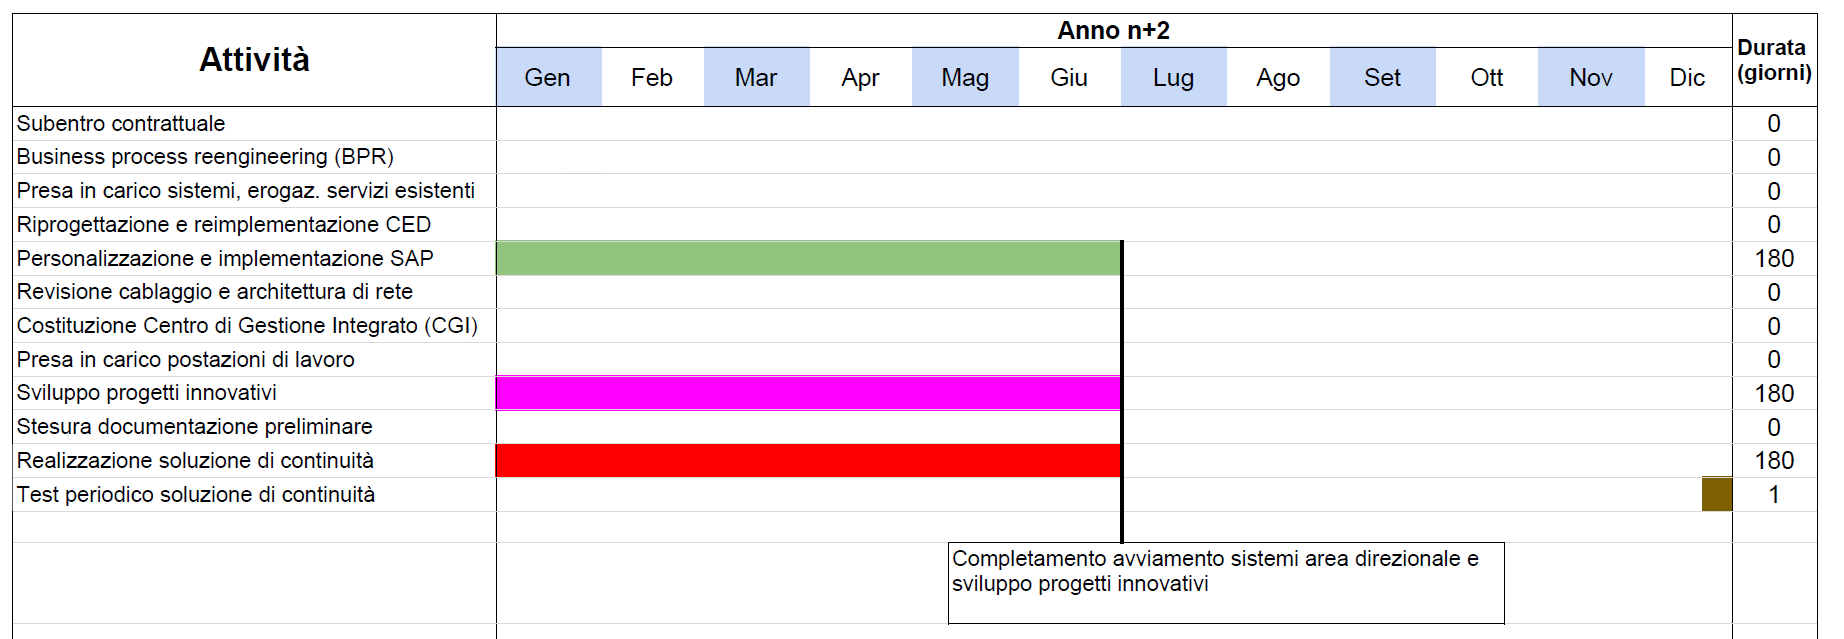
\includegraphics[width=\textwidth]{immagini/rollout/gantt-a3}
				\caption{Gantt anno n+2.}
			\end{figure}
                    
                    
		\subsection{Privacy e sicurezza}
                    In questa sezione verranno trattati requisiti, problematiche e soluzioni relative alla privacy e alla sicurezza durante la fase di rollout. In particolare, dato che durante la migrazione dai vecchi sistemi ai nuovi dovranno essere migrati anche i dati personali relativi ai dipendenti, il tema privacy assume un ruolo di fondamentale importanza.
                    
                    \subsubsection{Privacy}
                    
                    Dall'entrata in vigore del nuovo Regolamento sulla privacy del 25 maggio 2018 sono stati stabiliti obblighi stringenti e nuove responsabilità rispetto al precedente Codice della privacy con lo scopo di tutelare e salvaguardare i dati personali delle persone fisiche.
                
                
                	Il primo punto fondamentale da considerare è il \textbf{consenso} del soggetto di cui si stanno trattando i dati. Il consenso dev'essere sempre preventivo e inequivocabile, escludendo ogni ipotesi di consenso tacito. Dato che al momento della firma del contratto il Proponente tratta già i dati personali dei propri dipendenti, si presuppone che il consenso sia stato chiesto preventivamente all'assunzione. Tuttavia l'Offerente, in fase di migrazione, desidera confermare che tale consenso sia stato espresso in maniera esplicita, e sanando ogni discrepanza in caso non lo sia stato.
                    
                    
                    Il secondo punto da considerare è il \textbf{data breach}: in caso di violazioni esterne, come ad esempio attacchi hacker o furti di dischi, l'Offerente, in qualità di titolare del trattamento, dovrà comunicare il fatto al Garante nazionale e anche al soggetto interessato, nel caso in cui la violazione rappresenti una minaccia per i suoi diritti o le sue libertà. Sarà quindi necessario informare i membri del team dell'Offerente che verranno a contatto con dati personali di questa procedura, istruendoli sui passi necessari per trattare correttamente questo caso.
                    
                    
                    Come descritto nel regolamento, l'Offerente desidera seguire i principi di \textbf{privacy by default} e \textbf{privacy by design}. Secondo il primo principio, l'Offerente deve tutelare la privacy di default all'interno dell'organizzazione aziendale, dotandosi di sistemi opportuni. Per adempiere a ciò, l'Offerente memorizzerà i dati sensibiili all'interno di database protetti da password. La password verrà divulgata solamente ai soggetti che necessitano di conoscerla, seguendo il principio "\textbf{need to know}". L'accesso ai dati da parte di soggetti che non hanno bisogno di conoscere la password avverrà tramite apposite interfacce e maschere, con lo scopo di divulgare i dati personali nella minima quantità possibile.
                    
                    
                    Per quanto riguarda il secondo principio, \textbf{privacy by design}, il titolare dei dati deve proteggere i dati fin dalla progettazione di un applicativo o di un processo aziendale.  L'Offerente intende seguire in modo completo questo principio, progettando processi e applicativi di conseguenza. Per raggiungere questo scopo, si prevede un'analisi dei rischi legati al trattamento dei dati prima di eseguire le attività di progettazione. L'identificazione dei rischi sarà utile per evitare il verificarsi degli stessi.

					
                    Il Capo Progetto ricoprirà il ruolo di \textbf{Responsabile della Protezione dei Dati Personali (Dpo)}, data la sua grande esperienza e competenza, allo scopo di minimizzare i rischi dovuti al mancato rispetto del Regolamento sulla privacy.
                	
					\subsubsection{Sicurezza}
						Oltre alla privacy, un'altra componente che è necessario assicurare è la sicurezza. Dal punto di vista ITIL, la sicurezza (\textit{security}) è composta da:
                        \begin{itemize}
                        	\item \textbf{Confidentiality}.
                            \item \textbf{Integrity}.
                            \item \textbf{Availability}.
                        \end{itemize}
                        A differenza della privacy, che tende ed essere orientata ai processi, basata su ambito legale e la cui risposta alle violazioni è consiste tipicamente in una notifica, la security:
                        \begin{itemize}
                        	\item Si basa principalmente su ambito IT.
                            \item È orientata agli strumenti e alle tecnologie.
                            \item Risponde alle violazioni con contenimenti e correzioni.
                        \end{itemize}
                        L'Offerente, durante il rollout e la conduzione del progetto presso il Proponente, desidera seguire lo standard ISO 27001:2013 e seguenti, che documentano i requisiti e forniscono supporto per l'implementazione di un Information Security Management System (ISMS). Più nel dettaglio, ISO 27001 stabilisce che il management debba:
                        \begin{itemize}
                        	\item Sistematicamente esaminare i rischi di sicurezza.
                            \item Progettare e implementare meccanismi di controllo.
                            \item Adottare un processo di management globale.
                        \end{itemize}
                        L'adozione di un tale approccio permette l'identificazione tempestiva e la risoluzione dei rischi che rischiano di violare la sicurezza, aumentando contemporaneamente la credibilità nei confronti degli stakeholder.
                        Ulteriori dettagli implementativi esulano dallo scopo di questo documento e dovrebbero essere trattati dal processo di Information and Security Management (ISM).

\newpage

	\section{Supporto all'implementazione}
    	Questa sezione descrive le risorse necessarie per supportare l'implementazione, intese come hardware, software, strutture, materiali, documenti, personale e requisiti di formazione, rischi, problematiche e impatti implementativi sull'ambiente corrente.
        
        \subsection{Hardware, software e strutture}
			In questa sezione sono elencati hardware, software e strutture di supporto che l'Offerente utilizzerà l'implementazione del progetto. Più nello specifico, verranno indicati gli strumenti necessari all'Offerente per lo sviluppo delle soluzioni. Verranno tralasciati i modelli specifici per quanto riguarda l'hardware.
            \subsubsection{Hardware}
            	L'hardware necessario per l'implementazione è:
                \begin{itemize}
                	\item 10 PC di buone prestazioni per lo sviluppo degli applicativi (personalizzazioni SAP) e la stesura di documentazione.
                    \item 10 notebook di buone prestazioni per poter lavorare in mobilità.
                    \item Due server.   
                    \item Ulteriore hardware necessario all'implementazione della soluzione presso la sede del Proponente.
                \end{itemize}
                
            \subsubsection{Software}
            	Il software necessario per l'implementazione è:
            		\begin{itemize}
            			\item 20 licenze di Microsoft Office.
                        \item 20 licenze di Microsoft Windows 10.
                        \item 5 licenze Debian.
                        \item 5 licenze di kit di sviluppo software SAP per l'implementazione delle personalizzazioni.
                        \item 5 licenze Creately (sviluppo diagrammi UML).
                        \item Ulteriore software necessario all'implementazione della soluzione presso la sede del Proponente.
            		\end{itemize}
                    
            \subsubsection{Strutture}
            	Le strutture necessarie per l'implementazione sono:
               	\begin{itemize}
               		\item Sede dell'Offerente, con orari 9-13 e 14-18, lunedì-venerdì.
                    \item Sede del Proponente con orari 9-13 e 14-18, lunedì-venerdì.
               	\end{itemize}

			\subsection{Documentazione}
            	Durante l'implementazione del progetto sarà necessario produrre la seguente documentazione:
                \begin{itemize}
                	\item Organizzazione dei Processi Aziendali.
					\item Analisi sistemi.
					\item Piano di indirizzamento IP e di partizionamento della rete.
					\item Organizzazione Centro di Gestione Integrato.
					\item Progetti innnovativi.
					\item Documentazione quindicinale per documentare l'avanzamento del progetto.
                    \item Documenti di esito dei test annuali di continuità.
                \end{itemize}
                
			\subsection{Personale}
            	In questa sezione verrà descritto il personale necessario per l'implementazione del progetto.
                
                \subsubsection{Requisiti di staff}
                	Il personale richiesto per l'implementazione del progetto è il seguente:
                    \begin{itemize}
                    	\item 11 persone per la costituzione del Centro di Gestione Integrato presso la sede del Proponente.
                        \item 3 analisti.
                        \item 2 progettisti.
                        \item 3 programmatori.
                        \item 2 amministratori di sistema.
                        \item 2 ricercatori o dottorandi per analisi e brainstorming riguardo progetti innovativi.
                        \item 1 capo progetto.
                    \end{itemize}
				
                \subsubsection{Formazione dello staff}
                	\begin{itemize}
                		\item \textbf{Formazione staff Centro Gestione Integrato:} la formazione dello staff del CGI, che ricordiamo lavorerà stabilmente presso la sede del Proponente, verrà eseguito in maniera differente rispetto a quella degli altri membri del team. Dato che i membri del CGI devono rispondere efficacemente alle richieste degli utenti agendo da \textit{single point of contact} e affiancare il Proponente nella gestione quotidiana di vari compiti, l'Offerente desidera che il CGI sia costituito da personale altamente professionale. 
                        
                        
                        Allo scopo di formare questo personale, l'Offerente richiede che tutti i membri del CGI conseguano almeno la \textbf{certificazione ITIL Foundations} per dimostrare la propria conoscenza dei processi ITIL. Inoltre, saranno valutate positivamente altre certificazioni in campo informatico, come ad esempio la CompTIA A+. I membri saranno scelti tra candidati con buone capacità relazionali e soft skills, dando priorità a figure con esperienza pregressa in ruoli di service desk.
                        
                        
                        Ogni membro del CGI verrà messo a conoscenza dei processi aziendali del Proponente esistenti durante la presa in carico. Inoltre, prima della conclusione dell'attività di \textbf{Business Process Reengineering}, i membri del CGI verranno formati nuovamente, spiegando loro i nuovi processi.
                        
                        
                        L'Offerente sottoporrà ogni candidato membro del CGI ad un \textbf{test di valutazione}, sia in fase di presa in carico che prima della conclusione del BPR, per verificare la sua comprensione dei processi aziendali.
                        
                        
                        La formazione iniziale è stimata in 40 ore. Il personale del CGI continuerà ad essere formato anche dopo la presa in carico con regolari sessioni di formazione mensili, o straordinarie in caso di necessità. Allo scopo di rispettare gli SLA del service desk, le sessioni di formazione regolari saranno tenute dopo l'orario di lavoro, in modo da non lasciare il service desk completamente scoperto, compensando adeguatamente il personale.
                        
                        Le sessioni regolari di formazione, della durata di \textbf{1 ora}, seguiranno la seguente pianificazione:
                        \begin{itemize}
                        	\item Annunci: 5 minuti.
                            \item Discussione: 10 minuti.
                            \item Attività di soft skill: 15 minuti.
                            \item Formazione tecnica: 30 minuti.
                        \end{itemize}
                        
                        \item \textbf{Formazione di staff esterno al CGI:} l'implementazione del progetto richiede l'impiego di staff esterno al CGI, che consisterà in personale che lavora presso l'Offerente, già formato ed esperto nello sviluppo di soluzioni nell'ambito IT. Alla luce di questo, l'Offerente non prevede l'esecuzione di attività di formazione tecnica per lo staff esterno al CGI.


Tuttavia, ai fini di garantire il rispetto della privacy e della continuità, il personale verrà formato:
\begin{itemize}
	\item Inizialmente, con formazione di 20 ore, e continuativamente, ogni 6 mesi con sessioni di 2 ore, per la privacy.
    \item Continuativamente come indicato nella sezione \ref{ScadenzaContinuità} per la continuità.
\end{itemize}
\end{itemize}
                    
			\subsection{Rischi e problemi noti}
            	In questa sezione verranno esposti rischi, problemi, restrizioni o limitazioni che devono essere tenuti in considerazione durante lo sviluppo del progetto. Per i rischi verranno inoltre descritte delle contromisure che, da una prima analisi, risultano essere utili a diminuire il rischio residuo. 
                
                
                Nonostante questa sezione non voglia condurre un'analisi approfondita del rischio, obiettivo del processo di Risk Management, l'Offerente ritiene importante identificare i rischi che potrebbero impattare il processo di implementazione.
                
                \begin{figure}[H]
				\centering
				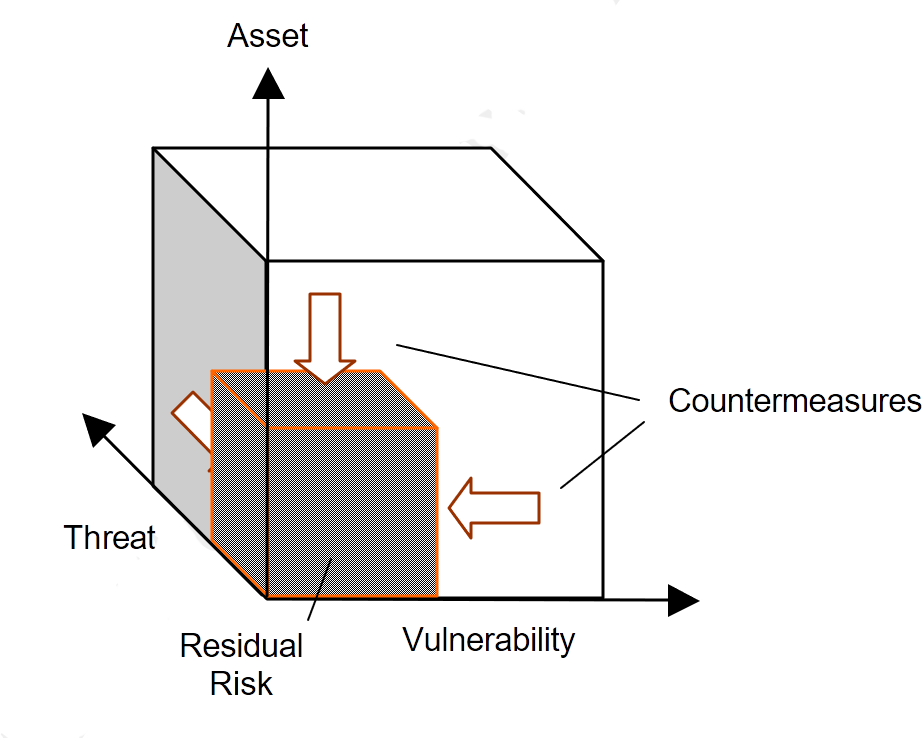
\includegraphics[scale=0.3]{immagini/rollout/risk}
				\caption{Rappresentazione del rischio (\url{https://goo.gl/iBomQ7}).}
			\end{figure}
                
                Ricordando la definizione di rischio definita dal \textbf{CRAMM}, ovvero il prodotto tra valore dell'\textbf{asset}, \textbf{minaccia} e \textbf{vulnerabilità}, nel seguito verrà svolta un'analisi semplificata, non tenendo in considerazione il valore dell'asset nel calcolo del rischio.
                
                
                Per ogni rischio verranno quindi specificati: 
                \begin{itemize}
                	\item \textbf{Livello di rischio}: indica il livello del rischio prima dell'adozione delle contromisure.
                    \item \textbf{Livello di rischio residuo:} indica il livello del rischio dopo l'adozione delle contromisure.
                \end{itemize}
                
                
                Adottando una misura qualitativa, ogni livello di rischio assumerà uno dei seguenti valori:
                \begin{itemize}
                	\item Alto: rischio alto, grave impatto sul business.
                    \item Medio: rischio medio, moderato impatto sul business.
                    \item Basso: rischio basso, piccolo impatto sul business.
                \end{itemize}
                
                
                \subsubsection{Ambiente ospedaliero}
                	È fondamentale tenere in considerazione che il team dell'Offerente dovrà implementare la soluzione progettata in un ambiente ospedaliero. Questo significa lavorare in un ambiente affollato, rumoroso e potenzialmente difficile da navigare. Il rischio maggiore è quello di intralciare le attività di medici e pazienti.
                    \begin{itemize}
                    	\item \textbf{Livello di rischio:} medio.
                        \item \textbf{Contromisure:} 
                        \begin{itemize}
                        	\item Informare medici e personale dell'ospedale delle attività che verranno eseguite.
                            \item Installare cartelli e altro materiale informativo nei pressi delle zone più pericolose, come il CED o corridoi molto frequentati.
                            \item Rispettare i regolamenti di sicurezza sul luogo di lavoro.
                            \item Eseguire le attività più "distruttive" in orari di bassa o nulla frequentazione, ad esempio evitando gli orari in cui sono permesse le visite.
                        \end{itemize}
                        \item \textbf{Livello di rischio residuo:} basso.
                    \end{itemize}
                    
				\subsubsection{Informazioni personali}
                	Come già descritto precedentemente, durante la migrazione l'Offerente verrà a contatto con informazioni personali di persone fisiche, ad esempio quelle del personale dell'ospedale e dei pazienti. Un eventuale data breach potrebbe avere conseguenze molto gravi, sia dal punto di vista legale che di immagine.
                    \begin{itemize}
                    	\item \textbf{Livello di rischio:} alto.
                        \item \textbf{Contromisure:} 
                        \begin{itemize}
                        	\item Limitare gli accessi ai dati sensibili seguendo il principio \textit{need to know}.
                            \item Proteggere i dati sensibili con password sicure.
                            \item Cambiare tali password una volta al mese.
                            \item Assicurarsi di limitare l'accesso fisico ai locali con apposite misure di sicurezza.
                            \item Controllare il background del personale che ha diritto all'accesso ai dati sensibili.
                        \end{itemize}
                        \item \textbf{Livello di rischio residuo:} medio.
                    \end{itemize}
                    
				\subsubsection{Interruzione del servizio}
                	All'Offerente viene richiesto di prendere in carico completamente la gestione del sistema informativo del Proponente, passando da una situazione frammentata con molti applicativi e sistemi ad una integrata, limitando il numero di questi elementi. Durante l'implementazione del progetto, e soprattutto durante la fase di migrazione dai vecchi sistemi al nuovo, c'è il rischio che si verifichi un'interruzione del servizio. Una tale eventualità potrebbe avere vari livelli di gravità, considerando le penali qualora si violassero gli SLA e anche i danni di immagine se l'interruzione dovesse causare danno a qualche paziente.
                    \begin{itemize}
                    	\item \textbf{Livello di rischio:} alto.
                        \item \textbf{Contromisure:} 
                        \begin{itemize}
                        	\item Pubblicizzare con largo anticipo (almeno 30 giorni) la data di migrazione da un sistema vecchio ad uno nuovo.
                            \item Concordare con il Proponente gli orari di down dei servizi per effettuare la migrazione.
                            \item Effettuare la migrazione quando tali servizi non sono in uso.
                            \item Sviluppare dei piani di rollback per ogni sistema nel caso in cui la migrazione non avesse successo.
                        \end{itemize}
                        \item \textbf{Livello di rischio residuo:} medio.
                    \end{itemize}
                    
				\subsubsection{Indisponibilità di risorse umane}
                	Per l'implementazione della soluzione sono necessarie le risorse umane indicate precedentemente. Il rischio riguarda la possibilità che alcune risorse umane non siano disponibili per qualche periodo a causa di motivi vari, come ad esempio problemi di salute. Se questa situazione si prolunga per lungo tempo si potrebbero avere ritardi di implementazione.
                    \begin{itemize}
                    	\item \textbf{Livello di rischio:} medio.
                        \item \textbf{Contromisure:} 
                        \begin{itemize}
                        	\item Attingere al personale residuo dell'Offerente, che si presume non starà lavorando sul progetto, in caso di indisponibilità di uno o più membri del team. Il personale di riserva dev'essere disponibile in misura del 10\% delle dimensioni del team.
                            \item Restare in contatto con candidati e agenzie di collocamento in modo da trovare dei sostituti in caso di indisponibilità di lungo periodo. 
                        \end{itemize}
                        \item \textbf{Livello di rischio residuo:} basso.
                    \end{itemize}
                    
				\subsubsection{Indisponibilità di risorse hardware}
                	Per lo sviluppo e l'implementazione della soluzione sono necessarie numerose risorse hardware, sia di proprietà dell'Offerente, utilizzate per lo sviluppo delle soluzioni, sia risorse nuove da acquistare, come postazioni di lavoro, switch, router e server. 
                    
                    
                    Il rischio consiste nell'indisponibilità di risorse sia per quanto riguarda l'Offerente, sia per quanto riguarda l'hardware che si deve acquistare.
                    \begin{itemize}
                    	\item \textbf{Livello di rischio:} medio.
                        \item \textbf{Contromisure:} 
                        \begin{itemize}
                        	\item Stipulare un contratto per la fornitura di hardware (postazioni di lavoro, server, ecc) a richiesta presso la sede dell'Offerente in tempi brevi (esempio: entro 24 ore).
                            \item Effettuare ordini di acquisto di hardware per la sede del Proponente con congruo anticipo.
                        \end{itemize}
                        \item \textbf{Livello di rischio residuo:} basso.
                    \end{itemize}
                    
                    
				\subsubsection{Ostilità e reticenza al cambiamento}
                    Il tipo di intervento richiesto dal Proponente è di profondo cambiamento sia dal punto di vista tecnologico che di processo. In questi casi non è raro incontrare reticenza al cambiamento da parte del personale del Proponente, specialmente se è abituato da molti anni ad un certo modo di lavorare.
                    
                    
                    L'Offerente necessita della massima collaborazione anche da parte del personale del Proponente, sia per quanto riguarda la conduzione di interviste per analizzare i processi esistenti, ma anche per organizzare al meglio il lavoro per non causare eccessivo disturbo.
                    
                    \begin{itemize}
                    	\item \textbf{Livello di rischio:} alto.
                        \item \textbf{Contromisure:} 
                        \begin{itemize}
                        	\item Pubblicizzare con largo anticipo i miglioramenti derivanti dall'adozione della nuova soluzione.
                            \item Impiegare personale con buone capacità relazionali e soft skills.
                            \item Fornire supporto fin da subito agli utenti.
                        \end{itemize}
                        \item \textbf{Livello di rischio residuo:} medio.
                    \end{itemize}

		\subsection{Impatto dell'implementazione}
        	In questa sezione verrà descritto come l'implementazione impatterà la realtà aziendale del Proponente, come ad esempio l'infrastruttura di rete e gli utenti. Verranno inoltre tenuti in considerazione gli SLA da rispettare durante l'implementazione.
            
            \subsubsection{Impatto sugli utenti}
            	L'implementazione del nuovo sistema avrà sicuramente un impatto sugli utenti. Sia che si tratti di personale medico o amministrativo, la rivoluzione applicativa e di processo andrà a cambiare radicalmente il loro modo di lavorare.
                
                
                Sarà necessario che, sopratuttto per i medici, l'impatto del nuovo sistema non riduca troppo le loro performance nell'esecuzione delle attività.
                
                
                Oltre a pubblicizzare il nuovo sistema, come indicato nella sezione precedente, l'Offerente intende effettuare dei rollout di tipo verticale durante la fase di test. Lo scopo di questi rollout avrà un duplice scopo:
                \begin{itemize}
                	\item Testare il sistema in un contesto limitato.
                    \item Abituare gli utenti all'utilizzo del nuovo sistema.
                \end{itemize}
                L'Offerente potrà raccogliere i dubbi principali degli utenti e redigere apposita documentazione sotto forma di Manuali Utente.
                        
			\subsubsection{Impatto sui pazienti}
            	Una delle richieste avanzate all'Offerente riguarda l'implementazione di un progetto innovativo per la creazione di PAN e l'informatizzazione del posto letto. Questo tipo di progetto va a coinvolgere in prima persona il paziente, con lo scopo di migliorare la sua esperienza durante il ricovero presso l'ospedale.
                
                
                Una corretta implementazione dei progetti relativi ai pazienti, che saranno anche loro utenti a tutti gli effetti, avrà senza dubbio un impatto positivo, a patto di non disturbare troppo la loro permanenza e di seguire le contromisure indicate nella sezione riguardo i rischi.
                        
			\subsubsection{Impatto sulla rete}
				L'Offerente si aspetta che la nuova soluzione richieda una banda di rete superiore rispetto a quella attualmente a disposizione del Proponente. Alcuni dei motivi dietro questo aumento sono: 
                \begin{itemize}
                	\item L'automazione di attività precedentemente eseguite manualmente.
                    \item  L'introduzione dei progetti innovativi.
                	\item L'esecuzione di più intensive e frequenti attività di backup, come previsto dal piano di continuità.
                \end{itemize}
                Alla luce di questo, il lancio di nuovi sistemi prima della messa in opera della nuova architettura di rete e del nuovo CED rischierebbero di gravare troppo sulla rete esistente, causando disservizi diffusi. 
                
                
                L'Offerente ha quindi pianificato, come da diagramma Gantt presentato precedentemente, il lancio dei nuovi sistemi solamente dopo la conclusione dei lavori sulla rete. Con questa accortezza l'impatto sulla rete dovrebbe essere minimo.
                
			\subsubsection{Impatto sugli SLA}
				L'implementazione della soluzione deve tenere conto degli SLA concordati con il Proponente. In riferimento a ciò, consideriamo l'indicatore globale riguardante la disponibilità delle soluzioni all'utente finale.                
				
                \begin{figure}[H]
				\centering
				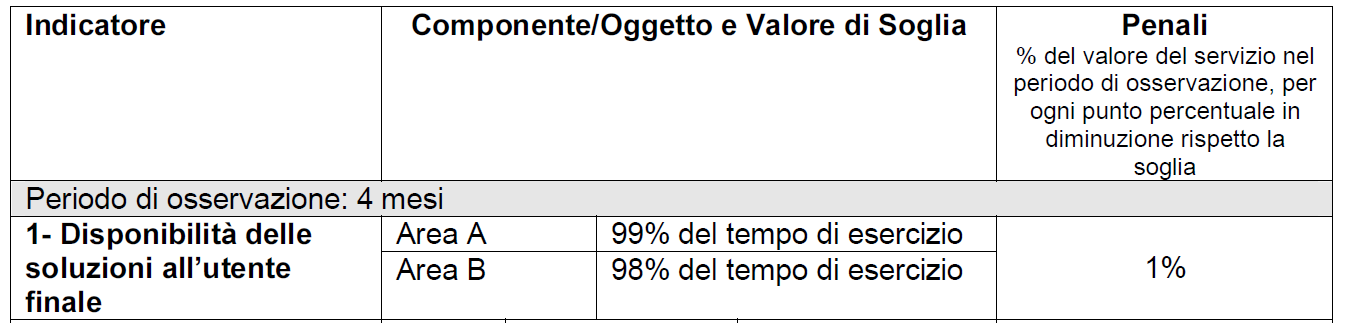
\includegraphics[scale=0.4]{immagini/rollout/sla1}
				\caption{Indicatore globale di servizio "Disponibilità delle soluzioni all'utente finale" (tratto dal Capitolato).}
				\end{figure}
                Considerando il periodo di osservazione di 4 mesi, e considerando una disponibilità pari a 40 ore settimanali in orario lavorativo, il downtime massimo accettato è di circa 6 ore ogni 4 mesi. Questo SLA fa capire che l'accensione dei nuovi sistemi non può permettersi di causare downtime.
                
                
                L'Offerente pianifica di avviare i nuovi sistemi e di eseguire tutte le manutenzioni necessarie in orario non di servizio. In ogni caso date e orari verranno stabilite di comune accordo con il Proponente.
                
		\subsection{Controllo delle performance}
        	Questa sezione descrive tool e tecniche per il monitoraggio e i modi con cui sarà possibile determinare se l'implementazione sta avendo successo.   
            
            
            Controllare periodicamente le performance dell'implementazione è fondamentale per assicurarsi di essere sulla giusta strada e correggere tempestivamente situazioni di errore prima che i problemi diventino troppo gravi. A questo scopo l'Offerente ritiene necessario l'utilizzo di \textbf{metriche} oggettive per la valutazione delle performance che quantifichino il raggiungimento o meno di certi obiettivi.
            
            
            Ad ogni metrica saranno assegnati dei \textbf{range di accettabilità} e di \textbf{ottimalità}, con il seguente significato:
            \begin{itemize}
            	\item Accettabilità: metrica accettabile ma non ottimale. Bisogna continuare ad osservarla con attenzione per rischiare che non degradi nella non accettabilità.
                \item Ottimalità: metrica ottimale, obiettivo pienamente soddisfatto.
            \end{itemize}
            Una metrica che assume un valore all'esterno di questi range non è accettabile e indica un obiettivo non raggiunto: sarà necessario contattare il Capo Progetto al più presto per stabilire delle misure correttive caso per caso. Per situazioni particolarmente gravi sarà necessario contattare il Coordinatore di Progetto (lato Proponente).
            

            \subsubsection{Soddisfazione del Proponente}
            	L'Offerente desidera che il Proponente sia soddisfatto durante tutta la durata dell'implementazione. La soddisfazione verrà misurata tramite dei sondaggi sottoposti mensilmente sia ai clienti che agli utenti, chiedendo loro di valutare in una scala da 1 a 10 la propria soddisfazione.
            	\begin{itemize}
            		\item \textbf{Range:} $[1, 10]$.
                    \item \textbf{Range di accettabilità:} $[6, 7]$.
                    \item \textbf{Range di ottimalità:} $[8, 10]$.
            	\end{itemize}
                Una valutazione insufficiente per più di due volte di seguito da parte dello stesso gruppo di interesse è da ritenersi un segnale d'allarme molto grave e richiederà attenzione immediata da parte del Capo Progetto.
			
            \subsubsection{Tempismo nell'esecuzione dei lavori}
            	L'Offerente desidera che l'esecuzione dei lavori rispetti il più possibile la pianificazione presentata nei Gantt della sezione \ref{sec:attivita} di questo documento. Un ritardo eccessivo potrebbe essere sintomo di problemi gravi non risolti, che rischiano di avere un effetto cumulativo sulle attività successive.
                
                
                Le rilevazioni sul tempismo verranno effettuate ogni due settimane, in coincidenza con la redazione della documentazione di avanzamento progetto da parte dei membri del team dell'Offerente.
                \begin{itemize}
            		\item \textbf{Range:} $[-\infty, +\infty]$ giorni.
                    \item \textbf{Range di accettabilità:} $[8,15]$ giorni.
                    \item \textbf{Range di ottimalità:} $[-\infty, 7]$ giorni.
            	\end{itemize}
                
                
			\subsubsection{Rispetto del budget}
            	L'Offerente desidera che il budget venga rispettato durante tutta l'esecuzione del progetto. Dato che la gestione del budget è legata intrinsecamente ad altre variabili, come qualità, portata e produttività, tenerla sotto controllo è fondamentale per il successo del progetto.

                
                Le rilevazioni sul budget verranno effettuate, come per la metrica precedente, ogni due settimane. Verranno indicate come scostamento percentuale rispetto al budget pianificato per quel periodo.
                \begin{itemize}
            		\item \textbf{Range:} $[-\infty, +\infty] \%$ .
                    \item \textbf{Range di accettabilità:} $[-10, -5), (+5, +10] \%$ .
                    \item \textbf{Range di ottimalità:} $[-5, +5] \%$ .
            	\end{itemize}
			\subsubsection{Rispetto degli SLA}
            	Rispettare gli SLA è fondamentale anche nella fase di implementazione: all'Offerente non è richiesta solamente l'implementazione di un progetto, ma la presa in carico e la fornitura di tutti i servizi IT del Proponente. Concentrarsi esclusivamente sull'implementazione della nuova soluzione e tralasciare la fornitura di servizi di qualità non è accettabile.

                
                Le rilevazioni per questa metrica verranno effettuate mensilmente, anche se il periodo di osservazione per gli SLA identificato nel capitolato risulta essere di 4 mesi. L'Offerente ritiene che misurare con questa frequenza possa dare risultati più tempestivi durante la fase di implementazione.
                \begin{itemize}
            		\item \textbf{Range:} $[0, +\infty]$ SLA violati.
                    \item \textbf{Range di accettabilità:} 0 SLA violati.
                    \item \textbf{Range di ottimalità:} 0 SLA violati.
            	\end{itemize}
                La soglia di accettabilità coincide con quella di ottimalità: questo significa che l'Offerente reputa anche solo la violazione di uno SLA non accettabile.
                

			\subsubsection{Risolvimento incidenti al primo livello}
            	Risolvere gli incidenti al primo livello di contatto (Service Desk) risulta essere fondamentale per non gravare eccessivamente sul personale tecnico, che risulta essere più proficuamente impiegato per l'esecuzione di attività di implementazione e manutenzione. 
                
                
                La rilevazione verrà effettuata su base mensile per tenere sotto controllo le performance del Service Desk.
                
                \begin{itemize}
            		\item\textbf{ Range:} $[0, 100] \% $ incidenti risolti al primo livello.
                    \item \textbf{Range di accettabilità:} $[70, 90] \%$ incidenti risolti al primo livello.
                    \item \textbf{Range di ottimalità:} $[90, 100] \%$ incidenti risolti al primo livello.
            	\end{itemize}
                
		\subsection{Gestione della configurazione}
        	Questa sezione descrive la gestione della configurazione da seguire durante l'implementazione del progetto.
            
            
            Nonostante un'analisi approfondita della gestione della configurazione, scopo del processo di \textbf{Service Asset and Configuration Management}, esuli dagli scopi di questo documento, l'Offerente ritiene utile presentare le metodologie e le convenzioni di massima che intende seguire durante il rollout.
            
            
            Ricordiamo che l'obiettivo del Configuration Management è di fornire un modello logico dell'infrastruttura attraverso l'identificazione, il controllo, la gestione e la verifica di tutte le versioni dei Configuration Items (CI) esistenti. Un CI è un'unità strutturale fondamentale di un sistema di gestione della configurazione. Alcuni esempi di CI sono: documenti, software e componenti hardware. I CI sono memorizzati all'interno di un database, detto CMDB.
            
              Per garantire la possibilità di identificazione univoca, ogni CI sarà identificato da:
              \begin{itemize}
              \item \textbf{ID:} identificativo univoco.
              \item \textbf{Numero di versione:} numero nella forma X.Y.Z che segue le norme del Semantic Versioning (\url{https://semver.org/}). In particolare
              \begin{itemize}
              \item \textbf{X}: numero di versione \textbf{major}, che indica un cambiamento radicale e incompatibile con le versioni precedenti del CI.
              \item \textbf{Y}: numero di versione \textbf{minor}, che indica un'aggiunta di funzionalità al CI compatibile con le versione precedenti.
              \item \textbf{Z}: numero di versione \textbf{patch/emergency}, che indica una risoluzione di problemi del CI compatibile con le versioni precedenti.
              \end{itemize}
              \end{itemize}
              Il numero di versione major 0 dev'essere utilizzato per i CI durante lo sviluppo iniziale. Dopo il go-live, i CI assumono numero di versione 1.0.0.
              
              
              L'Offerente prevede di rilasciare le major release esclusivamente con un approccio \textbf{push}. Questo approccio prevede che l'azione di ricevimento/installazione della release parta centralmente, avviata da parte dell'Offerente. Questa scelta è dovuta al fatto che le major release non sono retrocompatibili e l'Offerente reputa che la gestione di due o più CI con associate due major release diversi potrebbe essere fonte di inefficienze.
              
              
              Per quanto riguarda le minor e le patch/emergency release verranno rilasciate con un approccio \textbf{pull+push}. Questo approccio consiste nel rendere disponibile una release centralmente e permettere agli utenti di applicarla \textit{on-demand} quando lo ritengono necessario. Tuttavia, dato che non c'è garanzia alcuna sul fatto che gli utenti prelevino la release, l'Offerente si occuperà di rilasciare la release in modalità push dopo un certo limite di tempo, di norma una settimana ma variabile in base alla gravità e all'urgenza della release. Così facendo si uniscono i vantaggi della modalità push (rilasciare una release a tutti) a quella pull (dare la possibilità all'utente di scegliere il momento più opportuno per l'installazione).
              
              
		\subsection{Gestione delle sedi}
			La realtà aziendale del Proponente è strutturata su due presidi:
            \begin{enumerate}
            \item La Sede principale di Piazza Cardinal Ferrari.
            \item La Sede di Via Isocrate.
            \end{enumerate}
            L'Offerente si trova chiamato a formulare una strategia per gestire una situazione in cui è necessario effettuare un'implementazione e un rilascio multiplo su due sedi.
            
            
            Data la numerosità e la portata delle attività da eseguire, l'Offerente ritiene migliore adottare una strategia sequenziale piuttosto che parallela, che consiste nello svolgere un'attività prima sulla sede principale e poi sulla sede secondaria. 
            
            
            Seguire questo tipo di strategia porta i seguenti vantaggi:
            \begin{itemize}
            	\item Permette di concentrare maggiormente gli sforzi del team, evitando di disperderli su due realtà diverse.
                \item Permette di eseguire l'attività sulla seconda sede in maniera molto più efficiente, dato che si possono sfruttare gli effetti dell'apprendimento della prima sede, evitando quindi di compiere gli stessi errori due volte.
                \item Garantisce minori rischi dovuti a negligenza, data la maggior concentrazione durante l'esecuzione delle attività.
            \end{itemize}
            Tuttavia, seguire questo tipo di approccio in maniera estrema può portare al completare i lavori nella sede principale prima ancora di averli iniziati nella sede secondaria. L'Offerente vuole evitare questa situazione, dato che porterebbe ad avere sistemi inutilizzati per lungo tempo nella sede principale. La sequenzialità sarà quindi a livello di attività come descritte in sezione 3.2.2: una volta iniziata un'attività, verrà prima completata nella sede principale, e poi ci si concentrerà su quella secondaria. Il \textit{go-live} di sistemi e servizi verrà effettuato solo dopo il completamento dell'attività su entrambe le sedi.
            
              
		\subsection{Criteri di accettazione}
        	Questa sezione identifica i criteri di accettazione per la transizione dalla soluzione esistente alla nuova soluzione.
            
            
            In ognuna delle attività descritte dalla sezione \ref{sec:attivita} sono inclusi i criteri di accettazione per considerare quella specifica attività conclusa. Questa sezione si occupa dell'accettazione di livello più generale, concentrandosi quindi su sistemi e servizi.
            
            
            L'accettazione, anche detta validazione, viene eseguita dal processo di \textbf{Service Validation and Testing}. Il processo è composto dai seguenti sottoprocessi:
            \begin{itemize}
            \item \textbf{Definizione del modello di test:} specifica in dettaglio come la release verrà testata, definendo i \textit{test case} da utilizzare per la validazione.
            \item \textbf{Acquisizione delle componenti della release:} acquisisce le componenti di una release e valuta inizialmente, assicurandosi che solo le componenti che superano dei controlli di qualità stringenti possano essere testate in modo intensivo.
            \item \textbf{Test della release:} testa tutte le componenti e tutti gli strumenti e le tecniche richieste per l'implementazione, la migrazione e il \textit{back out} di una release. Solo le componenti che superano questi test possono entrare nell'ambiente live.
            \item \textbf{Test di accettazione del servizio:} verifica che sussistano tutte le condizioni affinchè il servizio possa essere attivato e ottiene il consenso da parte dell'utente che il servizio rispetta gli SLA concordati.
            \end{itemize}
           
           Seguendo quanto descritto da ITIL, prima del lancio di un servizio o di un sistema esso verrà testato sia internamente da parte dell'Offerente tramite test di unità, integrazione e sistema, sia esternamente, con la presenza del Proponente, in sede di collaudo tramite test di accettazione. 
           
           
           L'Offerente intende seguire l'approccio rappresentato dal seguente modello a V della Verifica e Validazione:
           
            \begin{figure}[H]
				\centering
				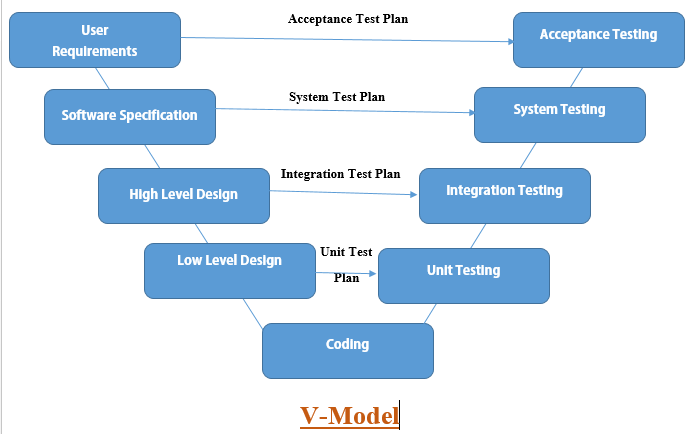
\includegraphics[scale=0.4]{immagini/rollout/v-model}
				\caption{Modello a V della Verifica e Validazione (\url{https://goo.gl/iHMCgV}).}
			\end{figure}
            L'Offerente ritiene fondamentale il successo della validazione esterna con il Proponente. Pertanto, al fine di assicurarsi il successo, verrà posta particolare attenzione all'esecuzione dei test di sistema in modo da certificarne la conformità complessiva.
            
            
            L'Offerente considererà sintomo di gravi problematiche un servizio o sistema che passa i test di sistema interni ma non quelli di accettazione. Qualora dovesse accadere, verranno contattati direttamente il Capo Progetto e il Coordinatore di Progetto per identificare le cause e trovare una soluzione di comune accordo.
            	
            
            
            
            
            
            
            
            
			
            
            
                







